\chapter{ConTrib: Preventing Free-riding Behaviour with Decentralized Micro-accounting}
\label{chapter2}

\emph{We present \ModelName{}, a universal accounting mechanism to prevent abuse in shared-resource systems.
%In contrast to existing work, \ModelName{} does not make assumptions on the connected applications.
In \ModelName{}, each individual maintains a personal ledger with \emph{records}.
%A serialized micro-record with an empty payload is only 275 bytes and efficient to transfer.
Micro-records describe past interactions and link to other ones, resulting in a global, interconnected graph.
Fraud, specifically the forking of ones personal ledger, is detected by participants themselves through the exchange and validation of micro-records.
We devise a system architecture and implement it.
Our evaluation shows that forking of a personal ledger can be detected within a minute and with reasonable bandwidth overhead.
We also find that that the throughput of \ModelName{} scales linearly with the network size.
To explore \ModelName{} in a realistic environment, we deploy our mechanism in a Tor-like overlay and show how free-riders are detected.
This trial has resulted in over 125 million micro-records, created by more than \TrialUsers{} users.}

\newpage

\section{Introduction}

% Big tech companies have an unprecedented amount of power

Preventing the abuse of resources is a key requirement in any shared-resource systems.
Often, such systems are safeguarded from abuse by having a single operator controlling every aspect of the system, essentially acting as a \emph{gatekeeper}.
Companies like Uber and AirBnb are prime examples of gatekeepers to marketplaces where user resources (e.g., cars and houses) are offered and consumed on a global scale.

%A key concern is that big tech companies retain full control over their deployed ecosystems and act as \emph{centralized gatekeepers}.
Even though the practice of acting as a central gatekeeper is widely adopted, it is a concerning development.
Recently, \enquote{big tech} companies have obtained significant dominance in the market for digital services.
Companies like Google, Amazon, Facebook and Apple are omnipresent in our current society and even have the means of acting as a small states, inhabited by billions of users worldwide.
%These companies continuously broaden their activities, often facilitating a large variety of digital services.
Unfortunately, this tremendous concentration of power allows for abuse of resources by the operator itself.
For example, it has been demonstrated that Uber actively manipulates the matchmaking process between passengers and drivers for commercial interests, therefore undermining fairness.
%Second, the long-term sustainability of the centralized gatekeeping model is questionable.
%Specifically, it poses systemic risks since a single decision by an operator can have far-reaching economic consequences for the platform.
%For example, the recent removal of Fortnite, one of the most popular games on the App Store, reduced the revenue of its publisher, Epic Games, by almost X\%.

%A key concern of these platforms is that they gain an unprecedented amount of control over the platform, resulting 
%Their ever-increasing market dominance has resulted in predatory behaviour, price discrimination, full platform control and winner-takes-all markets.
%Currently, the practices of many of these companies are under major antitrust investigation.

% Epic vs Apple?

Decentralized solutions are increasingly being explored as an alternative to shared-resource systems with centralized gatekeeping.
In contrast to centralized architectures, decentralized networks are fully maintained by participating peers without third-party supervision or central decision making.
In general, decentralized architectures tend to be more resilient against large-scale abuse of its resources.
However, peers in a sustainable decentralized system are required to fully coordinate the sharing of resources amongst themselves.
As such, preventing abuse in decentralized shared-resource systems is a problem that remains mostly unsolved.
%Yet, the detection of abuse is non-trivial since the relevant data might not be immediately available. % is dispersed across the network.
%However, the deployment of decentralized platforms poses new technical challenges that have to be addressed.
%These challenges include identity management, data availability, inducing cooperative behaviour amongst peers, and abuse management.

Recording resource consumption and contributions with an \emph{accounting mechanism} is a promising solution to address abuse in shared-resource systems.
Prior work aims to enhance decentralized systems with accounting mechanism, however, none of these solutions is universal enough to be reused across different application domains.
Blockchain technology provides accounting capabilities and empowers users with a distributed ledger to securely store their interactions. %, and financially remunerates users for securing the ledger.
Yet, blockchain is prohibitorily expensive to leverage for generic accounting since it requires large financial reimbursements to persist data in bulk.


%Since an operator has access to all historical events in a centralized system, detecting and addressing the abuse of resources is straightforward to achieve.
%This is more challenging in decentralized systems since information is dispersed across the network.

%\todo{bash centralized gatekeepers + antitrust}
%As a counterforce to the centralized architectures deployed by big tech companies, there has been significant effort to deploy decentralized systems that avoid third-party supervision.
%Blockchain technology, for example, empowers participants with a distributed ledger to securely record interactions and has been a key enabler of numerous decentralized systems like Bitcoin and Ethereum.
%Whereas the deployment of centralized systems is relatively straightforward, decentralized systems usually require additional complexity to mitigate the threats commonly found in decentralized networks.
%Significant research challenges include data availability and trust management.
%These threats include data unavailability, free-riding, and the Sybil Attack.

%\todo{alternative solution -> most feasible one is decentralized}
%\todo{prevent abuse in decentralized systems}

%At the heart of many systems, both centralized and decentralized, lies a mechanism for the secure storage and management of user-generated data.
%The storage and management of information in a decentralized system is a long-standing research challenge.
%Centralized service providers like Facebook and Amazon store all user data is stored on one or multiple servers that are fully under the control of the platform operator.
%On the other hand, secure and robust data management is considerably more challenging in decentralized networks where data must be stored by other, possibly untrusted peers.

%, with varying degrees of adoption.
%Perhaps the most influential example is Bitcoin, a digital currency that is fully maintained by its participating users.
%Bitcoin has demonstrated that it is possible to build a coin without banks.
%The core technology of Bitcoin, the distributed blockchain ledger, has bootstrapped much interest in decentralized alternatives.\todo{for example?}
%Another example is BitTorrent, a decentralized file-sharing protocol that enables users to directly exchange information.



%One might leverage blockchain technology to decentralized information management.
%Blockchain enables the tamper-proof and irrefutable storage of generic data elements, usually represented as transactions.

%Many of these innovations are pioneered by blockchain technology, which has been hailed as a panacea to disrupt these developments.
%Specifically, blockchain technology empowers users themselves to take on critical roles that are traditionally fulfilled by trusted authorities, e.g., banks, reshaping the notion of interactions in our society.
%Despite thriving ecosystems and markets worth billions of dollars (e.g., Ethereum), the first use case to pose a real threat to big tech companies has yet to be.
%This lack is mainly addressed to scalability limitations: blockchain technology is not performant enough yet to capture financial transactions on a global scale.

% The key challenge is to build a fully decentralized system, fully maintained by individuals. Requires adequate fraud prevention + free-riding prevention.

% One paragraph explaining how accounting in big-tech alternatives is different from existing work (e.g., PeerReview, Lifting, ...)

In this work, we introduce \ModelName{}, a universal accounting middleware to prevent abuse in shared-resource systems.
\ModelName{} enables tamper-proof storage of generic data elements within \emph{records}.
Records are the key building block of \ModelName{} and are linked together in a personal ledger.
%A micro-record describes an interaction from the perspective of one of the involved parties.
Users continuously share records with random users and validate incoming records against known ones.
%This enables quick detection of fraud, the illegitimate tempering of records.
Our simple, yet effective technique enables quick detection of fraud, specifically the situation where an adversary has forked its personal ledger and illegitimately modified a historical record.
We implement \ModelName{} and systematically evaluate its scalability and resistance against malicious users that undermine the accounting mechanism, e.g., by hiding or modifying the records in their personal ledger.
Our experiments with up to 1'000 users reveal that \ModelName{} that fraud can be detected well within a minute and that the throughput of \ModelName{} scales linearly with the network size.

To show the effectiveness and matureness of \ModelName{} in a realistic environment, we leverage our mechanism to record bandwidth traffic in \Tribler{}.
\Tribler{} is our academic peer-to-peer software and downloaded by over 1 million users.
Specifically, we use \ModelName{} to account bandwidth exchanges in our Tor-like overlay and refuse services to free-riders during periods of congestion.
Our 36-months measurements has resulted in over 120 million micro-records, created by over \TrialUsers{} users.
This large-scale deployment trial is a key milestone in our ongoing research to solve the tragedy-of-the-commons in Internet communities.

The main contribution of this work is four-fold:
\begin{enumerate}
	\item The universal \ModelName{} mechanism, suitable for the accounting of interactions in different shared-resource systems (Section~\ref{sec:micro_accounting} and \ref{sec:detecting_fraud}).
	\item A system architecture around \ModelName{} with flexible validity policies (Section~\ref{sec:system_architecture}).
	\item An implementation and evaluation of \ModelName{}, revealing fraud detection times within a minute and linear scalability (Section~\ref{sec:implementation_evaluation}).
	\item A large-scale deployment trial of \ModelName{} involving \TrialUsers{} volunteers, addressing bandwidth free-riding in a Tor-like overlay (Section~\ref{sec:deployment}).
\end{enumerate}

% We introduce ...

% Collective memory ...

%\section{Introduction}
%Free-riding, the act of selfishly benefiting from the usage of shared resources, is a common issue in both real-world and Internet communities~\cite{rose2003internet,adar2000free}.
%This selfish behaviour frequently prevails in Internet communities.
%This behaviour occurs when access to a shared resource is cheap and there are no individual consequences of overusing the good by community members.
%Structural free-riding on collective resources may result in a \emph{tragedy-of-the-commons}, the situation in shared-resource systems where the resource is depleted and the community around the resource collapses~\cite{hardin2009tragedy}.
%In this work, we address this behaviour by introduce a mechanism for digital shared-resource systems where all resource contributions and consumptions are accounted.
%Free-riding is a prevalent strategy within Internet communities.
%For example, digital media is aggressively competing for user attention, a scarce resource, through the unsolicited presentation of invasive banner ads and clickbait articles~\cite{chen2015misleading}.
%Ongoing Denial-of-Service (DOS) attacks on specific machines is another example of free-riding and shows that some individuals selfishly exploit the ubiquitous access to the Internet~\cite{cerf2013revisiting}.
%This behaviour shows that these attackers have a stronger incentive to undermine the security of shared Internet resources, rather than contributing to it.

%Shared-resource systems on the Internet are vulnerable to free-riding behaviour~\cite{locher2006free}.
%These systems are managing individuals with mutual access to computer resources offered to the community (e.g., bandwidth or CPU capacity).
%For example, downloading in the BitTorrent file-sharing network without contributing (seeding) back after the download has finished goes mostly unpunished and is therefore a common strategy~\cite{locher2006free}.
%Free-riding also occurs in anonymous networks like Tor, where users free-ride on the services offered by relay and exit nodes, without offering community services in return.
%Failure to acknowledge the presence of free-riding behaviour in peer-to-peer networks degrades the systems performance and could eventually result in users permanently leaving the network, as illustrated by the Gnutella software~\cite{adar2000free}.

%To date, the \emph{tragedy-of-the-commons} in Internet communities remains unsolved~\cite{harris2018institutional}.
%This social dilemma occurs where the community around a shared resource, e.g., storage capacity or bandwidth, will eventually collapse due to overexploitation when individual self-interest is at odds with community interests.
%A well-known example is \emph{free-riding} in file-sharing networks, where the act of downloading content without contributing (seeding) back after the download has finished goes mostly unpunished~\cite{locher2006free}.
%Long-term non-cooperative behaviour in shared-resource systems degrades the network performance and eventually leads to a community collapse as illustrated by peer-to-peer applications like  Gnutella~\cite{adar2000free}.

%The Internet has turned into a grim place, where selfish interest of big tech companies supersedes the importance of user-managed communities.
%Email spam is a prominent example of what happens when bandwidth is abused for selfish reasons.
%Over 45\% of email traffic consists of junk messages and an increasing number of ISPs and hosting providers are being forced to use sophisticated techniques in order to try at least to reduce it.
%Likewise, digital media is competing for user attention through the unsolicited presentation of invasive banner ads and clickbait articles.
%Ongoing DDoS attacks on specific machines show that some individuals have a stronger incentive to undermine the security of the Internet, rather than contributing to it.



%Oftentimes, the allocation of shared resources such as bandwidth is prescribed by the output of an algorithm that considers all historical contributions and consumptions of a peer~\cite{tang2004trust}.
%This trust can be based on historical action, or on a believe that the other agent will reciprocate a service later.
%Trade-based incentive mechanisms rely on remuneration for the volunteer resource sharing by agents, either through credits or monetary value.
%This is the approach taken by volunteer computing services, e.g., Boinc, and blockchain-based resource markets, e.g., FileCoin~\cite{benet2018filecoin} and Orchid~\cite{cannellorchid}.

%Providing meaningful incentives to reciprocate after taking some of its resources is imperative to alleviate free-riding behaviour and boost cooperating amongst participants~\cite{ma2004incentive}.
%Some shared-resource systems rely on a \emph{trade-based incentives} where resource consumption is immediately remunerated using a credit or payment system.
%For example, in many volunteer computing projects offered by BOINC users are rewarded for their contributed resources with virtual credits.
%Likewise, shared-resource systems build on blockchain technology leverage cryptocurrency payments to reward communal services~\cite{benet2018filecoin}.

%With \emph{trust-based incentives}, community members are indirectly reciprocated.
%Usually, the amount of provided and consumed resources to and from the community is expressed in a trust score, which can be computed by a reputation mechanism~\cite{meulpolder2009bartercast}.
%These scores are then used to determine a fair allocation of resources, for example, peers with a higher reputation are granted preferential treatment during periods of congestion.
%These trustworthiness scores can be computed by a reputation algorithm.
%To accurately determine the trustworthiness of individuals, shared-resource systems require a public accounting mechanism that records all interactions between users.
%This work focusses on secure accounting of interactions in such systems.

%There have been several proposals to address free-riding behaviour by securely accounting interactions~\cite{guerraoui2010lifting,haeberlen2007peerreview,mokhtar2014acting}.
%We find, however, that existing work is lacking in two directions.
%First, the design of existing solutions usually considers a specific application, e.g., file-sharing or gossip networks.
%This makes it hard, if not impossible, to re-use these solutions across shared-resource systems with differing resource types.
%Second, existing solutions tend to elevate the authority of specific peers in the network, e.g., by having a user act as witness for others.
%This introduces additional system complexities, e.g., incentivize users to not abuse their authority and to follow the protocol.

%As research points out, the interactions in digital shared-resource systems are usually short-lived and concern a small amount of resources~\cite{seuken2014work}.
%For example, the storage protocol FileCoin~\cite{benet2018filecoin} splits data into many small pieces and remunerate peers for the retrieval of individual pieces.
%Similarly, the BitTorrent file-sharing protocol orients around the transport of small data pieces with a variety of peers.
%Repeated, small interactions allows for lower risk-taking since peers can abort an interaction when its counterparty defects, e.g., when a counterparty goes offline during a file exchange.


%This approach aligns well with existing shared-resource systems where interactions are short-lived and concern a small amount of resources~\cite{seuken2014work}.
%For example, blockchain-based storage networks like FileCoin~\cite{benet2018filecoin} split data into small pieces and remunerate peers for the retrieval of pieces.
%Furthermore, micro-accounting allows for low risk-taking since peers can abort an interaction when its counterparty defects, e.g., when a counterparty goes offline during a file exchange.


%In this work, we design, implement, deploy and evaluate a 
%We identify two key advantages of micro-accounting

%So far, there is no lightweight and reusable \emph{micro-accounting} mechanism, specifically designed for recording small interactions in large shared-resource systems.

%Currently, there is no lightweight mechanism for tamper-proof accounting of community interactions, to the best knowledge of the authors.

% Motivate the need for micro-accounting
% 1) it aligns well with existing systems, e.g., file sharing and bandwidth sharing
% 2) it allows for quick punishment and blacklisting of users, with low value-at-risk

%So far, there has been a wide range of research in designing incentive-compatible mechanisms to prevent free-riding in decentralized networks.
%Many of the proposed models and mechanisms require secure accounting of community contributions, for example, if a peer has donated some storage to a specific peer or has uploaded a file to others.

%Most of these efforts are concentrated on reducing free-riding behaviour in file-sharing communities.
%However, free-riding is also prevalent in other communities, such as anonymity networks~\cite{biryukov2015proof}.
%We also observe that most research in this direction take a clean-slate approach for the implementation of their mechanisms.
%This leads to a large range of different implementations.
%Specifically, there is no universal, resource-agnostic infrastructure to quickly evaluate new mechanisms and policies.
%We argue that furthefr research on the management of Internet commons benefits from such an infrastructure.
%Many of these solutions share commonalities in the infrastructure required to deploy these mechanisms.

%\begin{figure}[b]
%	\centering
%	\includegraphics[width=\linewidth]{assets/components}
%	\caption{Our model for trust-based management of shared Internet resources such as bandwidth and storage.}
%	\label{fig:model}
%\end{figure}

%\begin{figure}[t]
%	\centering
%	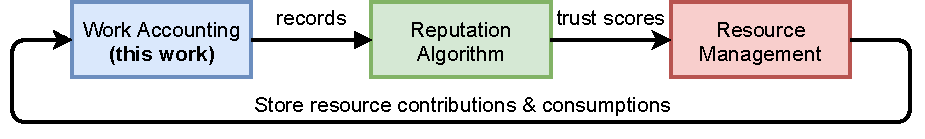
\includegraphics[width=\linewidth]{assets/trust_cycle}
%	\caption{Our envisioned approach to address free-riding behaviour in large-scale shared-resource systems.}
%	\label{fig:trust_cycle}
%\end{figure}

%We present \ModelName{}, a universal accounting mechanism for the detection of free-riding behaviour in shared-resource systems.
%Our mechanism enables resource accounting where fraud, e.g., illegitimate tempering of micro-records, can be efficiently detected across different shared-resource applications.
%\emph{Micro-records} are the key building block of \ModelName{} and are linked together in a personal ledger.
%A micro-record describes an interaction from the perspective of one of the involved parties.
%Users continuously share micro-records with random users and validate incoming micro-records against known ones.
%Our simple, yet effective technique enables quick detection of fraud, specifically the situation where an adversary has forked its personal ledger.
%We implement \ModelName{} and systematically evaluate its scalability and resistance against malicious users that undermine the accounting mechanism, e.g., by hiding or modifying the micro-records in their personal ledger.
%Our experiments with up to 1'000 users reveal that \ModelName{} that fraud can be detected well within a minute and that the throughput of \ModelName{} scales linearly with the network size.

%To show the effectiveness and matureness of \ModelName{} in a realistic environment, we leverage our mechanism to record bandwidth traffic in \Tribler{}.
%\Tribler{} is our academic peer-to-peer software and downloaded by over 1 million users.
%Specifically, we use \ModelName{} to account bandwidth exchanges in our Tor-like overlay and refuse services to free-riders during periods of congestion.
%Our 36-months measurements has resulted in over 120 million micro-records, created by over \TrialUsers{} users.
%This large-scale deployment trial is a key milestone in our ongoing research to solve the tragedy-of-the-commons in Internet communities.

%The \ModelName{} mechanism is based on two principles.
%First, we decouple the application logic and accounting primitives, unlike related work in the same domain~\cite{osipkov2006robust}.
%This results in a universal accounting mechanism that is reusable across different application domains.
%Second, \ModelName{} is specifically built to deal with the dynamic nature of peer-to-peer networks, where users quickly join or leave.
%Specifically, we avoid network-wide synchronization, group communication or the explicit management of witness sets, while ensuring that fraud will be detected with reasonable probability.

%This work is a cardinal part of our envisioned approach to solve the tragedy-of-the-commons, see Figure~\ref{fig:trust_cycle}.
%In this approach, peers account all resource contribution and consumptions within tamper-proof \emph{micro-records}.
%\ModelName{} records resource contributions and consumptions.
%Our envisioned next step is that every community member periodically runs a reputation algorithm on the collected micro-records which outputs subjective trustworthiness scores.
%These scores guide resource management, the process of determining which users will be granted access to some shared resource.

%Micro-records are organized in personal ledgers and can capture bilateral interactions between individuals by pointing to other micro-records.

%We identify the components and policies that together form an infrastructure for trust-based management of Internet resources.
%Our middleware is flexible, unlike blockchain-based approaches that require full replication and network-wide consensus.
%We build our middleware based on the model visualized in Figure~\ref{fig:model}.
%All community contributions are recorded on a light-weight and tamper-proof distributed ledger and used to compute trust scores by agents.
%These trust scores are then used to allocate resources to others.
%We identify, design and implement the required policies for the management of Internet resources in decentralized communities.

%We believe that the tragedy of the Internet commons can be solved through trust-based mechanisms.
%In this work, we build the required digital infrastructure and tools for sustainable community management on the Internet: accounting mechanisms, reputation algorithms, allocation policies.
%All presented components have been evaluated and tested through field trials with real users, using our academic software named Tribler.
%Tribler is the result of 15 years of engineering effort and has been downloaded by over 1.x million users.

% Possible system attacks:
% Free-riding
% Misreporting
% Collusion
% White-washing

\section{Problem Description}
\label{sec:problem_description}
The main challenge is to build a secure accounting mechanism for shared-resource systems.
We now elaborate on three requirements that our solution must adhere to.

\textbf{Requirement I: Full Decentralization.}
The information generated by our mechanism must be persisted somewhere.
Many shared-resource systems avert manipulation concerns by having a centralized manager store all credits or reputation scores of network participants (e.g., as in BOINC).
However, users now have to trust the manager that it does not modify the credit or trust scores.
As an alternative, one can leverage semi-decentralized solutions where a group of peers are responsible for the management of the system.
Blockchain, for example, is semi-decentralized since there is a group of peers of which the majority is assumed to be honest.

We require for our mechanism that all information is stored by users themselves.
Furthermore, we avoid any decision making by entities with leveraged authorities.
This makes our mechanism \emph{fully decentralized}.
In the context of this work, that means that all decisions are made by users, and there are no users with leveraged authority.
%For example, there have been various proposals to incentivize volunteer contributions to the Tor network by rewarding users with credits that are managed by a bank.
%In this scenario, the bank operator can gain an unfair advantage by minting its own credits.
In general, decentralized mechanisms are less vulnerable to large-scale attacks, tend to scale better, and are more resilient to failure.
They also are a good architectural fit with existing shared-resource systems without authorities, like BitTorrent~\cite{cohen2008bittorrent}.
%This requirement also implies that we aim to avoid peers with special permissions.

\textbf{Requirement II: Efficient Fraud Detection.}
In shared-resource systems where interactions are recorded, users have a natural incentive to misrepresent their prior information to inflate their social standing, or to hide information unfavourable to their standing~\cite{meulpolder2009bartercast}.
Therefore, our mechanism must ensure completeness and correctness of the stored information.
More specifically, we must \emph{detect the manipulation or hiding of recorded information} and punish the adversarial peers accordingly.
We consider misreporting, the inaccurate recording of interactions that have not actually occurred in the system, outside the scope of this work.
Misreporting should be taken into consideration by the reputation algorithm that processes the accounted interactions~\cite{seuken2010accounting}.
%Since different applications are likely to have differing visions on how fraud should be managed, we leave this decision to the application.

%For example, overuse in a file-sharing system can result in a temporary, e.g., 24-hour, ban or even result in ostracization from the community.

\textbf{Requirement III: Scalability.}
Open shared-resource systems on the Internet can grow to moderate or large sizes.
For example, applications like BitTorrent and Tor are used by millions of users.
We require that our solution \emph{scales} when the network size and number of interactions grow.

Blockchain technology is increasingly being used to manage shared-resource systems.
FileCoin, for example, is a decentralized system for renting out user-volunteered storage~\cite{benet2018filecoin}.
Participants in FileCoin record all interactions (data exchanges) within transactions on a distributed ledger, fully maintained by participants.
Transactions are bundled in blocks, and each block contains the hash of the prior block.
The modification of a transaction in one block is detected while reaching a distributed consensus.

Despite a growing ecosystem around the deployment of blockchain-based applications, blockchain technology have fundamental scalability limitations.
The key issue is that the network is required to continuously establish consensus on the entire transaction set~\cite{vukolic2015quest}.
%This consensus process is carried out by \emph{miners}, volunteers that manage the blockchain.
The need for consensus significantly limits the achievable throughput, and imposes high storage and bandwidth requirements.
The throughput of a blockchain secured by Proof-of-Work is usually limited to hundreds transactions per second at best, by far not sufficient to record interactions in large-scale shared-resource systems.
Furthermore, participants are required to store the full blockchain, which can grow to considerable sizes (e.g., the Bitcoin blockchain currently requires around 290 GB of storage).\footnote{See https://www.blockchain.com/charts/blocks-size}
We require a lightweight solution, suitable for deployment in large-scale networks.

%Scalability concerns are partially addressed by layer two solutions, e.g., state channels~\cite{mccorry2019pisa}.
%Transactions in layer two solutions are conducted off-chain and users maintain channels to route payment to other users. % users to create transactions 
%Yet, this technology still rely on a \enquote{primary} blockchain for channel management and dispute resolution.


%\textbf{Requirement III: Full decentralization.}
%Many shared-resource systems avert manipulation concerns by introducing a centralized manager that manages all credits or reputation scores of network participants (e.g., as in BOINC).
%However, users now have to trust the manager that it does not modify the credit or trust scores.
%Furthermore, a centralized manager complicates integration with existing systems since it introduces new roles and adds an additional dependency on external actors.
%In practice, dependency on a critical entity introduced a single point-of-failure since downtime of this entity stall all activity.

%As an alternative, one can leverage semi-decentralized solutions where a group of peers are charged with the system management.
%Blockchain is a semi-decentralized system since there is usually a group of peers of which the majority is assumed to be honest.
%Also, the PeerReview accounting mechanism uses witnesses to periodically inspect the correct behaviour of participants in the network~\cite{haeberlen2007peerreview}.

%This work specifically focusses on resource tracking in shared-resource systems.\todo{do something with this}
%There have been proposals to introduce accountability in distributed systems to either detect faulty behaviour or free-riding.

%Even though it is impossible to establish that the interaction embedded in a record has actually occurred, our micro-accounting mechanism should be able to handle record manipulation.

% Problem 1: detect manipulation
% Problem 2: avoid reliance on TTP

%\begin{figure*}[t!]
%	\centering
%	\begin{subfigure}[t]{.33\textwidth}
%		\centering
%		\captionsetup{width=.9\linewidth}
%		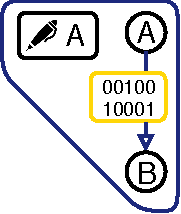
\includegraphics[width=.65\linewidth]{assets/tutorial_1}
%		\caption{To record an interaction between $ A $ and $ B $, $ A $ creates and sign a proposing micro-record (also called a \emph{proposal}).}
%		\label{fig:trustchain_tutorial_1}
%	\end{subfigure}%
%	\begin{subfigure}[t]{.33\textwidth}
%		\centering
%		\captionsetup{width=.89\linewidth}
%		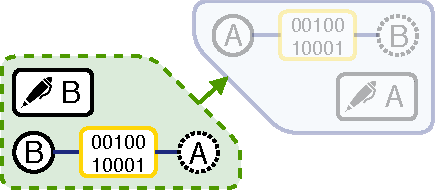
\includegraphics[width=.85\linewidth]{assets/tutorial_2}
%		\caption{Next, $ B $ confirms $ A $'s proposal by creating a confirming micro-record (also called a \emph{confirmation}), that points to it.}
%		\label{fig:trustchain_tutorial_2}
%	\end{subfigure}%
%	\begin{subfigure}[t]{.33\textwidth}
%		\centering
%		\captionsetup{width=.93\linewidth}
%		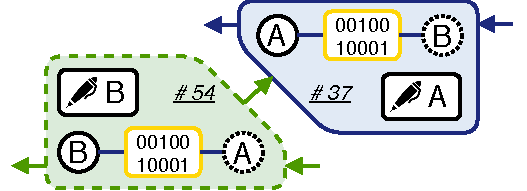
\includegraphics[width=.98\linewidth]{assets/tutorial_3}
%		\caption{To ensure tamper-proofness, we organize micro-records in personal ledgers and reference prior micro-records in a ledger.}
%		\label{fig:trustchain_tutorial_3}
%	\end{subfigure}
%	\caption{Storing an interaction between users $ A $ and $ B $ in \ModelName{} using two micro-records, one proposal and one confirmation. Solid and dotted circular elements indicate the identity of the micro-record creator, respectively, the micro-record counterparty.}
%	\label{fig:trustchain_tutorial}
%\end{figure*}

\section{\ModelName{} Design}
\label{sec:micro_accounting}
The design of our mechanism, named \ModelName{}, is inspired by the tamper-proof blockchain data structure, but avoids the need for network-wide consensus.
This allows to detect tampering while keeping the computational and bandwidth requirements low.
In \ModelName{}, each user maintains a personal ledger with \emph{micro-records} (see Section~\ref{sec:recording_interactions}).
These micro-records point to prior micro-records in the same personal ledger, and to micro-records in the personal ledger of others.
Users continuously share micro-records with other users.
By validating incoming micro-records against known ones, the manipulation of a personal ledger can now be detected.
Since micro-records are digitally signed by its creator, one can construct an irrefutable proof of some manipulation and share it with others.

In this section, we elaborate the design of \ModelName{} and the structure of micro-records.
First, we outline the system and threat model, and state the assumptions we make.
We then describe how an interaction is recorded in \ModelName{}.
%In \ModelName{}, an interaction indicates a small contribution or consumption of resources.
%The accounting of this interaction can proceed before or after the resources have been exchanged.

\subsection{System Model and Assumptions}
\ModelName{} is an accounting mechanism for shared-resource systems in which users share their computer resources, e.g., CPU power, bandwidth or files.
Our universal solution should record the interactions in multiple shared-resource systems simultaneously.

\ModelName{} leverages a peer-to-peer network in which users store their own micro-records and share micro-records with others.
We assume that each peer knows the network address of a subset of all peers.
The communication channels between peers are unreliable and unordered.
This means that the arrival time on messages is not upper bounded and messages could never arrive at the intended destination.
Each peer is in possession of a cryptographic keypair, consisting of a public and private key.
Their public key is used to uniquely identify the peer in the network, and the private key is used to digitally sign outgoing network messages.
We consider attacks targeted at the network layer, e.g., the Eclipse Attack, outside the scope of this work.

A key attack in peer-to-peer environments is the Sybil Attack, where an adversary operates multiple identities to either inflate its own social standing or to subvert the network~\cite{douceur2002sybil}.
This is a key issue in open Internet communities, where the cost of creating a new identity is often negligible.
In this work, we assume that this attack is solved either by leveraging semi-decentralized solutions for identity management, or by the reputation mechanism in Figure~\ref{fig:trust_cycle}.
Note that this does not violate our requirement for full decentralization since identity management is not a component of \ModelName{}.

\subsection{Threat Model}
\label{sec:threat_model}
Our threat model orients around malicious users that strategically manipulate their micro-records, either by sharing tampered micro-records or by withholding specific micro-records.
This attacks manifests by users operating on multiple copies of their personal ledger, possibly returning distinct micro-records to different users.
As discussed in Section~\ref{sec:problem_description}, our mechanism is required to detect this malicious behaviour.
We assume that the compute power of adversaries is bounded, that cryptographic primitives are secure and that digital signatures cannot be forged.
Our threat model also includes users that collude with other users to mislead other users.

%A particular treat is when peers collude in order to record false information, e.g., a bandwidth upload that has not actually occurred within the system.
%It is non-trivial to verify whether the interaction has actually occurred in the system and therefore, we consider this attack outside our scope.
%Addressing this attack likely requires a mechanism that leverages application-specific properties.
%For example, TorPath builds a proof-of-bandwidth that proves that some bandwidth has been transferred through a circuit~\cite{ghosh2014torpath}.
%Creators of fake information should be given a lower trust score by the reputation mechanism, as illustrated in Figure~\ref{fig:trust_cycle}.

%Users store dual-signed agreements of their interactions using \ModelName{} in \emph{micro-records}.

%\begin{table}
%\begin{center}
%	\begin{tabular}{ | p{1cm} | p{6.5cm} | }
%		\hline
%		\textbf{Field} &\textbf{Description} \\
%		\hline
%		$ i $ & The index of the micro-record in the personal ledger of $ a $. \\
%		$ a_{pk} $ & The public key of $ a $. \\
%		$ b_{pk} $ & The public key of $ b $. \\
%		$ t $ & The type of the micro-record. \\
%		$ p $ & The payload of the micro-record. \\ 
%		$ s_{a,i} $ & A digital signature by $ a $ over the micro-record. \\ 
%		$ h_{a,i-1} $ & The hash of the previous micro-record in the personal ledger of $ A $. \\ \hline
%		$ l $ & The index of the referenced proposal. \\ 
%		$ h_{b,l} $ & The hash of a referenced proposal. \\
%		\hline
%	\end{tabular}
%\end{center}
%\caption{The fields in a micro-record created by user $ a $, capturing an interaction with user $ b $. A proposal does not contain the last two fields ($ l $ and $ h_{b,l} $).}
%\label{tab:micro_record}
%\end{table}

\begin{figure}[t]
	\centering
	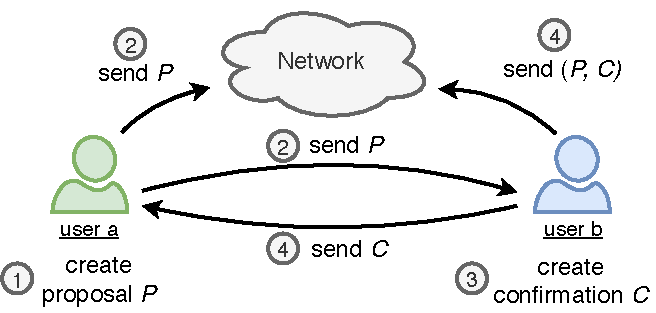
\includegraphics[width=\linewidth]{trustchain/assets/interaction}
	\caption{Recording an interaction between two users ($ a $ and $ b $) using two micro-records (proposal $ P $ and confirmation $ C $).}
	\label{fig:interaction}
\end{figure}

\subsection{Recording Interactions}
\label{sec:recording_interactions}
\ModelName{} resolves around users creating \emph{micro-records}.
A micro-record contains information on an interaction between two users.
%Each micro-record is either a \emph{proposal} or a \emph{confirmation}.
An interaction between users $ a $ and $ b $ is recorded using two micro-records: one \emph{proposal} created by $ a $ and one \emph{confirmation} created by $ b $.

We outline how an interaction between users $ a $ and $ b $ is recorded, and elaborate on the structure of both types of micro-record.
This process is visualized in Figure~\ref{fig:interaction}.
First, $ a $ creates a proposal, which we refer to as $ P $ (step \circled{1}).
$ P $ contains the public key of both $ a $ and $ b $, a type, a payload, and a digital signature over the micro-record content, generated with the private key of the creator.
The type field is a short string identifier that allows multiple applications to leverage \ModelName{} simultaneously.
The payload of the payload is an arbitrary blob of data and is provided by the application.
To increase the resilience against manipulation, we extend micro-records with additional fields later.
%A transaction is a generic description of any interaction between users, for instance, making an agreement or recording a trade.
%We consider a transaction to be the result of \emph{any} interaction between users, like transferring assets or recording agreements. %We intentionally consider a transaction to be a description of any interaction between two users.
% As a result, it can describe almost every interaction between two or more users, like asset transfers or generic agreements.
After $ a $ included all described fields in the proposal, the micro-record is persisted to $ a $'s database, sent to interaction partner $ b $ for confirmation, and disseminated to $ f $ random users (step \circled{2} in Figure~\ref{fig:interaction}).
We refer to $ f $ as the \emph{fanout}.

%A micro-record created by user $ a $, capturing an interacting with $ b $ is defined as a tuple $ R_{a,i} = (i, a_{pk}, b_{pk}, t, p, s_{a,i}, h_{a,i-1}, l, h_{b,l}) $.
%All fields in $ R_{a,s} $ are listed and described in Table~\ref{tab:micro_record}.
%Every micro-record is equipped with a sequence number $ i \in \mathbb{Z} $ that indicates the index of the micro-record in the personal ledger of the creating user.
%It also contains the public keys of both interacting users.
%A micro-record created by $ a $ contains a hash pointer ($ h_{a,i-1} $) to the previous micro-record in the personal ledger of $ a $.

When $ b $ receives the proposal $ P $, $ b $ verifies its validity.
The validation logic of micro-records is explained in detail in Section~\ref{sec:detecting_fraud}, and invalid micro-records are dropped.
If the incoming proposal $ P $ is valid, $ b $ determines if the payload in $ P_a $ describes the correct interaction details.
If not, $ b $ ignores the incoming proposal.
Otherwise, $ b $ creates a confirming micro-record, denoted by $ C $, that confirms the proposal and links to it (step \circled{3} in Figure~\ref{fig:interaction}).
This confirmation contains the same fields as the proposal $ P $ and also includes the hash of $ P $.
We call the hash pointer to the linked proposal in a confirmation the \emph{confirmation pointer}.
After the creation and signing of $ C $, $ b $ persists the confirmation to its database, sends it to $ a $, and disseminates both the proposal and confirmation to $ f $ random users (step \circled{4}).
Upon reception of $ C $, $ a $ validates and persists $ C_b $ if it is valid.
Both parties are now in possession of the proposal and confirmation that together prove an interaction between these parties.
This process is non-blocking since users can engage in the recording of multiple interactions with different interaction partners at the same time.
This ensures liveness of \ModelName{}, even when the counterparty refuses to confirm a proposal or goes offline.

%The encoding format of the payload $ p $ depends on the application in which the interaction has taken place.

%The creator of the micro-record digitally signs the micro-record and includes the signature.
%It also confirms that both parties agree with the transaction itself.
%Digital signatures can be effectively verified by others.

%To ensure that micro-records are replicated in the network when $ A $ or $ B $ goes offline, each new micro-record is disseminated to $ f $ random users in the network by default.
%We refer to $ f $ as the fanout.
%Each transaction has a \emph{type} field, indicating its purpose.
%Blocks are linked together by a (hash) pointer that points to the prior block in each individual ledger.
%Both transacting parties digitally sign the transaction they are involved in by using any secure digital signing algorithm (TrustChain uses the ECDSA algorithm).
%These digital signatures are included in a block, which ensures that participation by both parties is irrefutable.
%It also confirms that both parties agree with the content within the transaction.
%Others can efficiently verify digital signatures in blocks since the digital identities of both interacting parties (their public keys) are also included in a block.
%After all required signatures have been added to a block, the block is appended to the individual ledgers of the two interacting parties and committed to their local databases.
%TrustChain also allows unilateral transactions without any counterparty.
%The block with a unilateral transaction is only signed by the issuing party and then committed to their individual ledger.

A potential risk is that $ b $ refuses to confirm $ P $, even though the incoming proposal is valid and contains the correct interaction details.
This could, for example, happen when confirming $ P $ negatively impacts $ b $'s social standing.
This leaves $ a $ with an unconfirmed proposal, which alone is not sufficient evidence to convince other users of the interaction between $ a $ and $ b $.
In this situation, $ a $ will add $ b $ to a local blacklist, refusing to share resources until $ b $ has confirmed $ P $.
To minimize the loss for $ a $ in this situation, shared-resource systems using \ModelName{} should frequently record interactions.
%Since the interactions in connected shared-resource applications should be of low value, $ a $ has contributed minimal resources to $ b $ without being accounted, which is likely to be an acceptable loss for $ a $.

%Note how the blockchain structure in Figure \ref{fig:trustchain_tutorial_2} allows user $ A $ to modify blocks in their individual ledger without being detected by others.
%In particular, $ A $ can reorder the blocks in its individual ledger since validity can quickly be restored by recomputing all hashes.
%In most blockchain applications, the global consensus mechanism prevents this kind of manipulation.
To prevent the modification of created micro-records, we organize all micro-records of the same user in a tamper-evident \emph{personal ledger}.
Each user now maintains and grows their own personal ledger with micro-records.
Specifically, we extend each micro-record with an additional hash pointer that points to the prior micro-record in the personal ledger of the creator, incrementally ordered by creation time.
The modification of a micro-record now also changes the hash of subsequent micro-records, making it easier to detect modifications.
To index a micro-record in a personal ledger, each micro-record includes a sequence number $ s \in \mathbb{Z} $ that is incremented by one when a new micro-record is created.
The confirmation pointer now also includes the sequence number of the proposal that it confirms.
This structure sets the \ModelName{} data structure apart from traditional blockchain structures, where the entire network maintains a single chain with transactions.
The structure of \ModelName{} is more comparable with DAG-based blockchains, e.g., IOTA~\cite{popov2018tangle}.
%A key difference, though, is that \ModelName{} does not require network-wide consensus on all stored records.
%Each block now has exactly two incoming and two outgoing (hash) pointers, except for the last block in an individual ledger, which only has two incoming pointers.

In addition to the hash pointer of the prior block, each micro-record also includes at most $ n $ additional hash pointers to distinct, prior micro-records in the same personal ledger.
Intuitively, this enables quicker detection of tampering in a personal ledger since an inconsistency in the hash of micro-records can be faster detected.
We further elaborate on this in Section~\ref{sec:detecting_fraud}.
The micro-records that a specific micro-record must point to, is deterministically given by a function $ \sigma $ that takes a public key and sequence number as input.
This function returns a set with at most $ n $ sequence numbers.
All users must use the same implementation of $ \sigma $, which can be achieved by including the implementation of $ \sigma $ in the \ModelName{} software.
We call the set of hash pointers that link to previous micro-records in the same personal ledger the \emph{prior pointers}.

\begin{figure}[t]
	\centering
	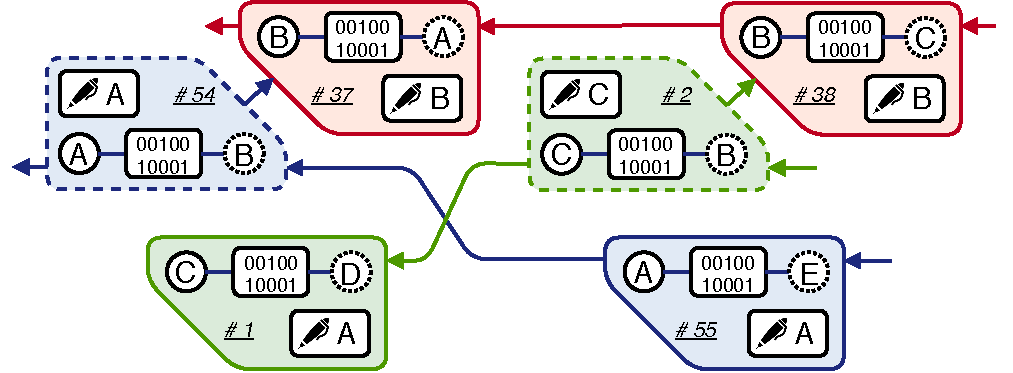
\includegraphics[width=\linewidth]{trustchain/assets/fullchain}
	\caption{A part of the \ModelName{} DAG with five users and six micro-records: four proposals and two confirmations (indicated by dashed borders). The proposal created by user $ A $ is unconfirmed.}
	\label{fig:fullchain}
\end{figure}

The creation and confirmation of micro-records yields the graph structure as shown in Figure \ref{fig:fullchain}.
Figure \ref{fig:fullchain} shows a part of the \ModelName{} structure with six micro-record, created by three distinct users.
Micro-records in the same personal ledgers have the same colour, and confirmations are dashed.
For presentation clarity, we only show the hash pointer to a prior block in ones personal ledger.
The micro-record in $ a $'s personal ledger with sequence number 55 is unconfirmed.
When two parties transact and create a micro-record, their personal ledgers essentially become intertwined, or \enquote{entangled}.
The process of recording interactions is non-blocking, lightweight and avoids network-wide consensus: recording a bilateral interaction only requires two digital signatures and the exchange of two micro-records.
%This property makes fraud impractical to hide since a counterparty is able to proof malicious activities by revealing his block with the disputed transaction.

\subsection{Recording multilateral interactions}
The current design of \ModelName{} orients around the recording of bilateral interactions.
Arguably, this is sufficient for most shared-resource applications where interactions are between two users.
However, recording an interactions between $ n > 2 $ parties can be achieved by one party creating a proposal and the other parties confirming this proposal, requiring $ n $ micro-records in total.
Each micro-record is modified so that it contain the public keys of all interaction partners.
Furthermore, each new confirmation should point to the proposal and the confirmations already made by the other interaction partners.

\begin{figure*}[t!]
	\centering
	\begin{subfigure}[t]{.33\textwidth}
		\centering
		\captionsetup{width=.9\linewidth}
		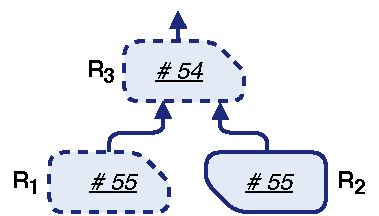
\includegraphics[width=.65\linewidth]{trustchain/assets/fraud_scenario_1}
		\caption{\emph{Scenario I}: $ R_1 $ and $ R_2 $ violate the integrity constraints of the personal ledger, providing an irrefutable proof of fraud.}
		\label{fig:fraud_scenario_1}
	\end{subfigure}%
	\begin{subfigure}[t]{.33\textwidth}
		\centering
		\captionsetup{width=.89\linewidth}
		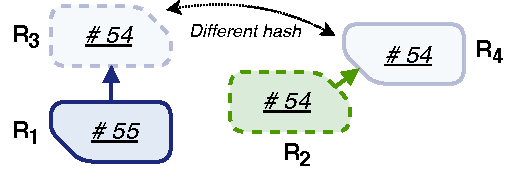
\includegraphics[width=.9\linewidth]{trustchain/assets/fraud_scenario_2}
		\caption{\emph{Scenario II}: $ R_1 $ and $ R_2 $ point to a micro-record with the same sequence number and creator, but a different hash. This reveals an inconsistency.}
		\label{fig:fraud_scenario_2}
	\end{subfigure}%
	\begin{subfigure}[t]{.33\textwidth}
		\centering
		\captionsetup{width=.93\linewidth}
		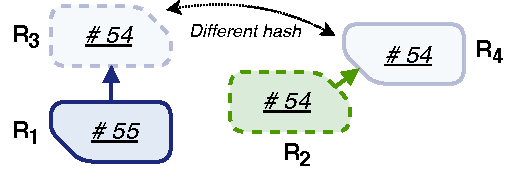
\includegraphics[width=.98\linewidth]{trustchain/assets/fraud_scenario_3}
		\caption{\emph{Scenario III}: $ R_1 $ and $ R_3 $ confirm a micro-record with the same sequence number and creator, but a different hash. This reveals an inconsistency.}
		\label{fig:fraud_scenario_3}
	\end{subfigure}
	\caption{Different scenarios which allows a user to expose a fork, or detect suspicions of fraud attempts. The colour of each micro-record indicates the identity of its creator (blue for $ a $, green for $ b $ and red for $ c $). Solid and dashed micro-records indicate proposals, respectively confirmations. Opaque micro-records are not in possession by the user.}
	\label{fig:fraud_scenarios}
\end{figure*}

\section{Detecting Fraud}
\label{sec:detecting_fraud}
As discussed in Section~\ref{sec:problem_description}, we require that \ModelName{} detects malicious tampering of the micro-records in a personal ledger.
\ModelName{} is built around fraud \emph{detection} instead of \emph{prevention}.
We argue this is a reasonable assumption for two reasons.
First, shared-resource systems can usually tolerate low amounts of fraud for short time periods~\cite{krishnan2002virtual}.
Second, preventing fraud is a resource-intensive process that requires users to reach a consensus on all created micro-records, e.g., using classical BFT algorithms or Proof-of-Work~\cite{vukolic2015quest}.
In \ModelName{}, fraud management proceeds on the application level, where a shared-resource application could, for example, decide to refuse services to the fraudster for some time.

%First, we highlight how an adversary would commit fraud in \ModelName{}.
Fraud in \ModelName{} proceeds when an adversary branches (or forks) its personal ledger and operates multiple personal ledgers, possibly with a common prefix of micro-records.
This fraud, for example, happens when an adversary aims to hide a specific micro-record by replacing it with another one.
This would result in pairs of micro-records with the same sequence number that have the same backward pointer, but a different hash.
%This fraud model aligns with related work on free-riding behaviour in peer-to-peer networks~\cite{haeberlen2007peerreview}.

%According to our threat model, manipulation in \ModelName{} involves an adversary maintaining two different personal ledgers, possibly with a common prefix.
%In related literature, this is often referred to as double-spending or chain forking.

%To incentivize users to participate in the exploration of the \ModelName{} DAG, we propose that collected fraud proofs can be given to resource providers to gain preferential treatment.\todo{elaborate}
%For example, a user $ A $ can modify, reorder or remove micro-records in their personal ledger, and recompute the hash pointers to restore validity.
%However, this basic manipulation can be proven by interaction partners of $ A $ by having them broadcasting the original and manipulated micro-records created by $ A $ with the same sequence number.

%To prove this fraud to others, a user can broadcast the original and manipulated micro-records.

\subsection{Detecting Forks}
The forking of ones personal ledger is detected by disseminating new micro-records to random users, and by continuously requesting existing micro-records from other users.
We will further discuss the dissemination of micro-records in Section~\ref{sec:exchanging_records}.
%In \ModelName{}, users continuously request micro-records in the personal ledger of other users, and the micro-records that confirm the requested micro-records.
Incoming micro-records are verified against known micro-records in the users' database to detect multiple copies of ones personal ledger.
This enables efficient fraud detection through the collective effort of users.
When a user refuses to send requested micro-records to a requester within reasonable time, the requester blacklists that user and refuses to share resources with that user.
Due to our network assumptions, we remark that requested micro-records can arrive in any order.

In Figure~\ref{fig:fraud_scenarios}, we highlight three scenarios in which we can either expose an adversarial user (scenario I), or detect an inconsistency without exposing the adversarial user yet (scenario II and III).
Each scenario shows a (subset) of micro-records that a single user knows or does not know (these micro-records are faded).
Micro-records with the same colour are created by the same user.
The first scenario, visualized in Figure~\ref{fig:fraud_scenario_1}, shows a part of the personal ledger of a user $ a $.
This personal ledger is forked since micro-record $ R_1 $ and $ R_2 $ have the same public key and sequence number.
As soon as another user, say $ b $, receives $ R_1 $ while already having $ R_2 $, or receives $ R_2 $ while already having $ R_1 $, the pair $ (R_1, R_2) $ is sufficient evidence to prove that $ a $ has forked its personal ledger.
Note that $ b $ does not require $ R_3 $ to detect or prove this fraud.
We call this pair a \emph{fraud proof}, which are by default shared with other users upon its detection.

%The other two scenarios, displayed in Figure~\ref{fig:fraud_scenario_2} and Figure~\ref{fig:fraud_scenario_3}, enables the detection of an inconsistency but one cannot assign blame without more context.
Figure~\ref{fig:fraud_scenario_2} shows the scenario where a user receives proposal $ R_1 $ and already has confirmation $ R_2 $, or receives confirmation $ R_2 $ while already having proposal $ R_1 $.
The user does not have $ R_3 $ and $ R_4 $.
The hash pointer to the prior micro-record in $ R_1 $ differs from the hash pointer in the confirmation $ R_2 $.
This indicates an inconsistency that is either introduced by user $ a $ forking its personal ledger at height 54, or by $ b $ having included an invalid hash pointer in $ R_2 $.
A user that encounters this situation during the validation logic optimistically sends the pair $ R_1 $ and $ R_2 $ to $ f $ other users to hopefully determine which user is to blame.

Figure~\ref{fig:fraud_scenario_3} highlights another scenario where a user encounters two confirmations ,$ R_1 $ and $ R_3 $, created by different users, that point to a micro-record with the same public key and sequence number, but a differing hash.
This either indicates a fork of the personal ledger of $ a $, or it can be the result of an invalid pointer in one of the confirmations.

%A more advanced manipulation is \emph{forking}, where a user creates two micro-records with the %same sequence number but with different counterparties.
%The goal of this fraud is to hide a specific micro-record from ones personal ledger, e.g., records that indicate some resource consumptions.
%This is similar to the double-spend attack in blockchain ledgers like Bitcoin~\cite{grunspan2018double}.
%Only when a user discovers both conflicting micro-records, this manipulation can be proven.
%In Section~\ref{sec:fraud_detection_experiment} we demonstrate that this fraud can be detected within seconds.
%To prove this fraud, the transaction counterparty reveals both the correct block and the invalid block created by $ A $.

% Rewrite prior intersactions themselves
Two users, say $ a $ and $ b $, may collude in order to modify prior micro-records, which is valid according to our threat model (see Section~\ref{sec:threat_model}).
We remark that when both users refrain from disseminating the micro-records after their creation, both users can still agree to change or remove the micro-records.
However, when the micro-records have been disseminated to other users, any modification to these micro-records can now be proven by other users.

\begin{algorithm}[b]
	\label{alg:record_validation_step2}
	\caption{Comparing the fields of an incoming micro-record against a known one.}
	\begin{algorithmic}[1]
		\Procedure{validateAgainstKnown}{r}  \Comment{Step 2}
		\State differs = False
		\State stored $ \leftarrow$ db.get(r.publicKey, r.seqNum)
		\If{!stored}
		\State differs = True
		\EndIf
		\If{r.type $ \not= $ stored.type}
		\State differs = True
		\EndIf
		\If{r.payload $ \not= $ stored.payload}
		\State differs = True
		\EndIf
		\If{r.linkPublicKey $ \not= $ stored.linkPublicKey}
		\State differs = True
		\EndIf
		\If{r.linkSeqNum $ \not= $ stored.linkSeqNum}
		\State differs = True
		\EndIf
		\If{r.linkHash $ \not= $ stored.linkHash}
		\State differs = True
		\EndIf
		\If{r.signature $ \not= $ stored.signature}
		\State differs = True
		\EndIf
		\If{r.hash $ \not= $ stored.hash}
		\State differs = True
		\EndIf
		
		\If{differs = True}
		\State \textsc{shareFraudProof}(r, stored)
		\EndIf
		
		\State \Return differs
		
		\EndProcedure
		
	\end{algorithmic}
\end{algorithm}

\subsection{Micro-record Validation Logic}
\label{sec:validation_logic}
Given our fraud detection mechanism, we now present the validation logic of an incoming micro-record $ r $.
To simplify the validation logic, proposals and confirmations have the same fields.
The confirmation pointer is implemented with three fields: \textsc{linkPublicKey}, \textsc{linkSeqNum} and \textsc{linkHash}.
In a proposal, these fields are set to \textsc{null}.
Each user maintains a dictionary \textsc{hashes} with known hashes.
%Upon receiving a new micro-record, \textsc{validateRecord} is invoked with the incoming micro-record.

The validation logic is broken down in five steps.

\textbf{Step 1.}
First, we verify the validity of the fields included in $ r $, without considering other micro-records.
This is performed by the \textsc{validateRecordFields} function, which returns a boolean value indicating if the checks during this step passed.
Its implementation can be found in Appendix~\ref{sec:validation_record_data}.
This step includes a verification of the included public key, the sequence number and the digital signature.
Any error in the included fields of the incoming micro-record is computationally efficient to detect and is likely the result of a software bug.

\textbf{Step 2.}
Next, we query the database for a micro-record with the same public key and sequence number as $ r $.
If such a micro-record exists, say $ r' $, we compare the fields of $ r $ with the fields in $ r' $.
This is performed by the \textsc{validateAgainstKnown} method given in Listing~\ref{alg:record_validation_step2}.
If any field in $ r $ differs from $ r' $, we have detected a fork in ones personal ledger and share the fraud proof with the network.

\textbf{Step 3.}
Next, we compare the incoming micro-record $ r $ with its counterpart.
If $ r $ is a proposal or confirmation, we verify the accompanying confirmation and proposal, respectively.
This step is performed by the the \textsc{validateLink} method given in Listing~\ref{alg:record_validation_step3}.
This step specifically validates the hash pointer to the micro-record in the personal ledger of the interaction counterparty.
For example, it checks whether the pointed micro-record contains correct back-links to the incoming micro-record.
This verification allows the detection of scenario III visualized in Figure~\ref{fig:fraud_scenario_3}.

\textbf{Step 4.}
Next, we verify if the incoming micro-record is consistent with other micro-records in the same personal ledger.
This is performed by the \textsc{validateChainLinks} method which implementation is given in Listing~\ref{alg:record_validation_step4}.
This method first fetches the previous and next micro-record in a personal ledger, and then checks the pointers.

\textbf{Step 5.}
Finally, we verify the validity of the included payload, which is an application-dependent validation procedure.
As we will further outline in Section~\ref{sec:system_architecture}, shared-resource applications using \ModelName{} should implement a \emph{validation} policy that denote whether the payload of an incoming micro-record is valid in the context of the application.

\begin{algorithm}[t]
	\label{alg:record_validation_step3}
	\caption{Validating a micro-record against a linked micro-record.}
	\begin{algorithmic}[1]
		\Procedure{validateLink}{r}  \Comment{Step 3}
		\State linked $ \leftarrow$ db.getLinked(r)
		\If{!linked}
		\State \Return True
		\EndIf
		\If{r.linkPublicKey $ \not= $ linked.publicKey \textbf{and} r.publicKey $ \not= $ linked.linkPublicKey}
		\State \Return False
		\EndIf
		\If{r.seqNum $ \not= $ linked.linkSeqNum \textbf{and} r.linkSeqNum $ \not= $ linked.seqNum}
		\State \Return False
		\EndIf
		\If{r.isConfirm}
		\If{r.linkHash $ \not= $ linked.hash}
		\State \Return False
		\EndIf
		\State linkLinked $ \leftarrow $ db.getConfirmLinked(link)
		\If{linkLinked \textbf{and} linkLinked.hash $ \not= $ r.hash}
		\State \Return False
		\EndIf
		\EndIf
		\EndProcedure
	\end{algorithmic}
\end{algorithm}

\subsection{Exchanging Micro-Records}
\label{sec:exchanging_records}
Detecting forking of ones personal ledger requires adequate strategies to exchange micro-records with others.
We distinguish between a \emph{push-based} and a \emph{pull-based} exchange of micro-records.

\textbf{Push-based Exchange.}
With a push-based exchange, the creator of a micro-record disseminates it to $ f $ random users.
As discussed in Section~\ref{sec:recording_interactions}, if the interacting parties follow the protocol, they will push the created micro-records to other users.
This push-based exchange allows for quick detection of forking since the probability of no user receiving two conflicting micro-records quickly goes to zero, even when the network is of considerable size~\cite{osipkov2007combating}.
Furthermore, immediately disseminating a micro-record in the network ensures replication in the network when its creator goes offline.
Users that purposefully operate multiple personal ledgers, however, are less likely follow the protocol and aim to hide the conflicting micro-records.
In Section~\ref{sec:fraud_detection_experiment} we show that forking is still detected, even when no user broadcasts created micro-records.

\textbf{Pull-based Exchange.}
It is not guaranteed that forks are eventually detected when using a push-based exchange.
Therefore, each user by default also requests (pulls) micro-record from other random users.
When answering such a request, users also respond with the proposal or confirmation that links to the requested micro-records, if available.
When a user $ a $ does not answer with micro-records within reasonable time, a requesting user adds $ a $ to a local blacklist.

\begin{figure*}[t]
	\centering
	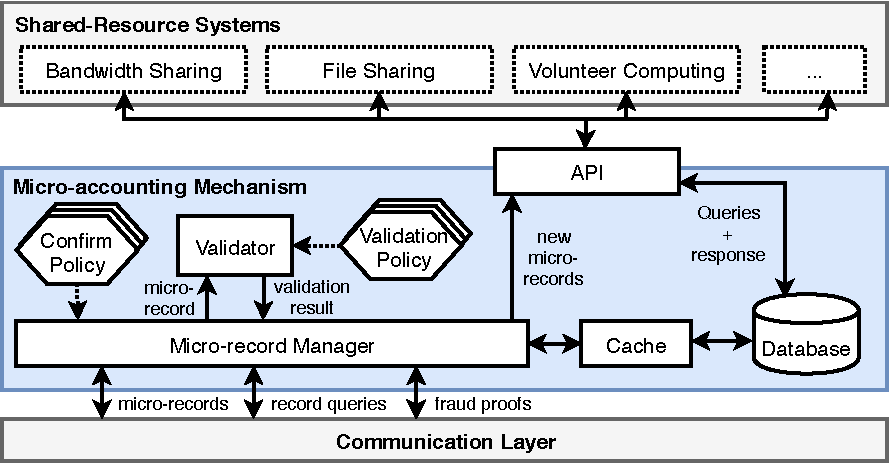
\includegraphics[width=\linewidth]{trustchain/assets/system_architecture}
	\caption{The system architecture of \ModelName{}.}
	\label{fig:system_architecture}
\end{figure*}

\begin{algorithm}[t]
	\label{alg:record_validation_step4}
	\caption{Validating the back-pointer of an incoming micro-record.}
	\begin{algorithmic}[1]
		
		\Procedure{validateChainLinks}{rec}  \Comment{Step 4}
		\State prevRec $ \leftarrow $ db.get(rec.publicKey, rec.seqNum - 1)
		\State nextRec $ \leftarrow $ db.get(rec.publicKey, rec.seqNum + 1)
		\If{prevRec \textbf{and} prevRec.hash $ \not= $ rec.prevHash}
		\State \Return False
		\EndIf
		\If{nextRec \textbf{and} nextRec.prevHash $ \not= $ rec.hash}
		\State \Return False
		\EndIf
		\EndProcedure
		
	\end{algorithmic}
\end{algorithm}

\section{System Architecture}
\label{sec:system_architecture}
%We present the components of our middleware, which is visualized in Figure~\ref{fig:system_architecture}.
%We consider peer-to-peer communities without centralized server.
%We also deem threats at the network layer, such as the Sybil Attack and the Eclipse Attack, outside scope of this work.

%\subsection{Underlying Model for Resource Management}
%Figure~\ref{fig:model} shows the underlying model of our middleware.
%This model is inspired by prior work on deterring free-riders in BitTorrent networks based on reputation, and consists of three components~\cite{seuken2010accounting,meulpolder2009bartercast}.
%An \emph{accounting mechanism} (see Section X) stores all resource contributions and consumptions by agents.
%These actions are embedded in tamper-proof and light-weight records, and shared with other individuals in the network.
%Each individual collects records from others, eventually building a local database.
%These records are then passed to a \emph{reputation algorithm} that determines the trustworthiness of individuals it knows about.
%Even though accounting mechanisms and reputation mechanisms share similarities, they are incomparable as discussed in the work of Seuken et al.~\cite{seuken2010accounting}.
%There exists a large number of decentralized reputation algorithm.
%The output of the reputation algorithm is a mapping from the identity of individuals to a trust score.
%These trust scores are used by the \emph{allocation policy} to provide access to some common good.
%The interactions following the allocation are accounted and public, and influence subsequent trust scores.
%For example, if a peer $ A $ downloads from another peer $ B $, the trust score of peer $ B $ most likely increases whereas the scores of peer $ A $ decreases.

We devise a system architecture around our \ModelName{} data structure (see Figure~\ref{fig:system_architecture}) and elaborate its components.
%We also demonstrate how resource-sharing applications can leverage the described system architecture and leverage \ModelName{} for resource accounting.
Communication primitives are the lowest layer in our system architecture.
This layer can be realised using existing frameworks to build peer-to-peer overlay networks, e.g., libp2p.\footnote{https://libp2p.io}
%Mitigation of network threats, e.g., the Sybil and Eclipse attacks, should be addressed by the communication layer.

\textbf{Micro-record Manager.}
The micro-record manager has a coordinating role in the \ModelName{} system architecture.
It interacts with the communication layer to disseminate micro-records and to process incoming micro-records.
It queues incoming micro-records for validation and persists incoming fraud proofs to the database.
It also manages the confirmation of incoming, valid proposals that are targeted at that user.
Applications using \ModelName{} should implement \emph{confirmation policies} that predicate whether an incoming proposal should be confirmed.
This decision is likely dependent on application-specific data.
%When micro-records arrive from the network, the record manager first checks if it has been received before.
%If not, it schedules the micro-record for validation.

\textbf{Micro-record Validator.}
The validator assesses the validity of incoming micro-records according to the logic outlined in Section~\ref{sec:validation_logic}.
%We distinguish between validation on \emph{record-level} and \emph{data-level}.
%Validation on record-level verifies the whether the micro-record itself is valid, e.g., whether it contains a valid digital signature and whether the micro-record is in alignment with other known micro-records in the personal ledger.
%These validation rules are application-agnostic.
%Validation on data-level verifies integrity of the micro-record with respect to an application context.
%Note that the validator might not have sufficient information to validate an incoming micro-record on data-level and therefore must collect more micro-records first.
Developers can implement different \emph{validation policies} for micro-records with differing types.
If implemented, the appropriate validation policy is invoked during step 5, when the payload is validated.
The flexibility to provide validation and confirmation policies for different micro-record types makes \ModelName{} universal and reusable across different application domains.

%\begin{algorithm}[b]
%	\SetAlgoLined
%	\small
%	\KwData{Micro-record \emph{R}, database \emph{db}}
%	\lIf{$ R $.$sequence\_number < 1 $}{\Return{} \textbf{false}}
%	\lIf{f}{\Return{} \textbf{false}}

%	\caption{The validation of a micro-record}
%\end{algorithm}

\textbf{Persistence.}
Micro-records and fraud proofs are persisted in a database.
The \ModelName{} system architecture provides an interface for the queries made to the database and therefore supports different database architectures, e.g., structured or unstructured storage models.
All query databases by \ModelName{} are routed through a \emph{micro-record cache}, which is an intermediary component that pre-loads all micro-records in the personal ledger of the operating user.
This allows \ModelName{} to quickly respond to incoming requests.
%Micro-records of ones own personal ledger are cached in an intermediary \emph{record cache} in order to quickly respond to incoming queries.
%The record cache stores intermediate records for quick lookup when receiving a query for micro-records in ones personal chain.
%When initiating \ModelName{}, it pre-loads the micro-records of the operating user in the cache.
The micro-record cache interacts with the database for the retrieval and storage of micro-records and fraud proofs.

To limit the growth of the database, we periodically prune the database when it stores a certain number of micro-records (in our implementation, we start pruning at 1 million micro-records).
The default pruning strategy of \ModelName{} continuously removes the micro-record with the lowest insertion timestamps, until the database has reached its storage threshold.
The pruning of older micro-records from the database might cause some forks to go undetected, since micro-records are removed before a fraud proof can be constructed.
However, as we will show in Section~\ref{sec:fraud_detection_experiment}, forks in \ModelName{} are quickly detected and there should be ample time to detect inconsistencies before the pruning process kicks in.

\textbf{Fraud Management.}
When the validator exposes fraud, or when it receives an incoming fraud proof, the connected applications are notified of the event and can punishment the misbehaving user accordingly.
For example, a fraud policy in a bandwidth sharing application could decide to not serve the fraudster for some time and refuse resources to the adversarial user.

Despite enforcing a temporal order in a personal ledger, there is no notion of physical event time in \ModelName{}.
Even if we would extend micro-records with a timestamp field, there is no guarantee that the included timestamp is accurate.
%This inaccuracy prevents resource-sharing applications using \ModelName{} to utilize time-based policy, e.g., banning adversarial users for 24-hours after the moment the fraud has been committed. % have committed fraud.
In a distributed system with Byzantine actors, it is not practically possible to accurately synchronize time.
Even though we consider accurate timestamping of events out of scope, we briefly outline two solutions.
One approach is to use Proof-of-Work mechanisms to implement a distributed timestamp service.
However, this approach is resource intensive and there would still be inaccuracies in the produced timestamps.
Alternatively, one can use a third-party timestamping service and include their signature in the payload of a micro-record.
However, this would violate our requirement for full decentralization, as discussed in Section~\ref{sec:problem_description}.

\textbf{Interacting with \ModelName{} by Applications.}
Shared-resource systems interact with \ModelName{} through an API.
This API allows applications to query the content of the database used by \ModelName{}.
Furthermore, connected applications can subscribe to incoming micro-records with a specific type.
The micro-record manager forwards new micro-records to the API, which passes the micro-records to subscribed application.

\begin{figure*}[t]
	\centering
	\begin{subfigure}{\columnwidth}
		\centering
		
\includegraphics[width=\linewidth]{trustchain/assets/fraud_experiments_legend}
	\end{subfigure}
	\begin{subfigure}{.66\columnwidth}
		\centering
		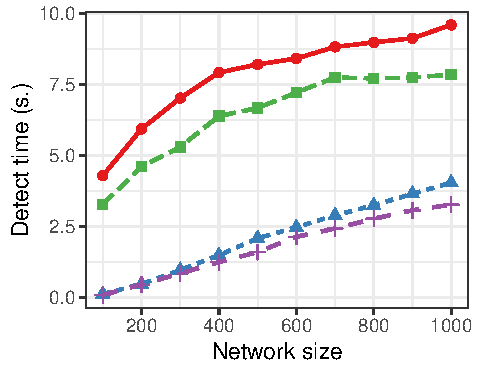
\includegraphics[width=\linewidth]{trustchain/assets/fraud_experiment_fixed_tx}
		\caption{Fraud detection times}
		\label{fig:fraud_experiment_fixed_tx_time}
	\end{subfigure}%
	\begin{subfigure}{.66\columnwidth}
		\centering
		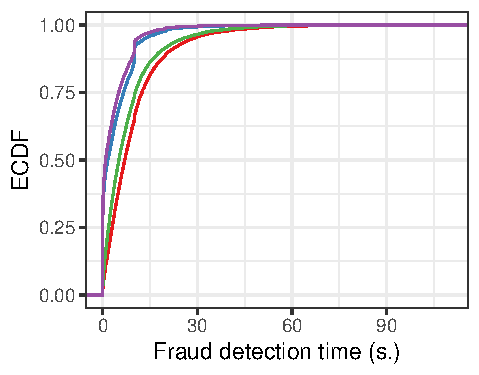
\includegraphics[width=\columnwidth]{trustchain/assets/fraud_experiment_detect_times_fixed_1000}
		\caption{Fraud detection times ($ n = 1'000 $)}
		\label{fig:fraud_experiment_detect_times_fixed_1000}
	\end{subfigure}
	\begin{subfigure}{.66\columnwidth}
		\centering
		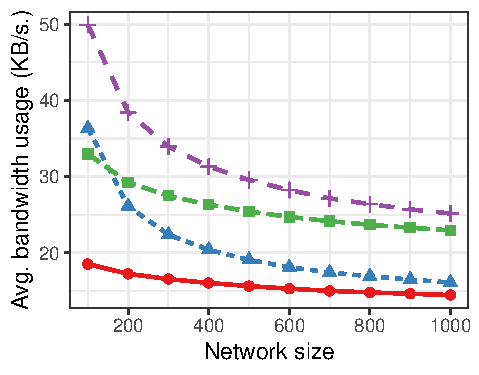
\includegraphics[width=\columnwidth]{trustchain/assets/fraud_experiment_fixed_tx_bw}
		\caption{Bandwidth usage}
		\label{fig:fraud_experiment_fixed_tx_bw}
	\end{subfigure}%
	\caption{The fraud detection times and bandwidth usage of \ModelName{} while recording 100 interactions per second. $ n $ indicates the network size. We fix the fanout to 10.}
	\label{fig:fraud_experiments_fixed_tx}
\end{figure*}

\begin{figure*}[t]
	\centering
	\begin{subfigure}{\columnwidth}
		\centering
		
\includegraphics[width=\linewidth]{trustchain/assets/fraud_experiments_legend}
	\end{subfigure}
	\begin{subfigure}{.66\columnwidth}
		\centering
		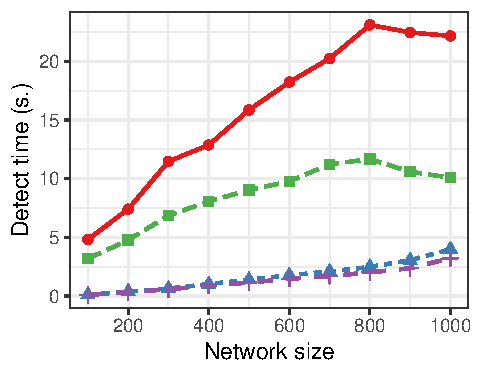
\includegraphics[width=\linewidth]{trustchain/assets/fraud_experiment_dynamic_tx}
		\caption{Fraud detection times}
		\label{fig:fraud_experiment_dynamic_tx_time}
	\end{subfigure}%
	\begin{subfigure}{.66\columnwidth}
		\centering
		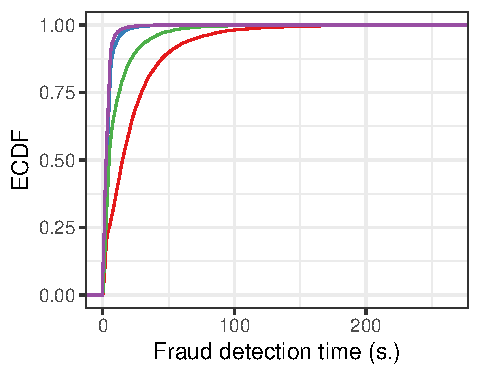
\includegraphics[width=\columnwidth]{trustchain/assets/fraud_experiment_detect_times_dynamic_1000}
		\caption{Fraud detection times ($ n = 1'000 $)}
		\label{fig:fraud_experiment_detect_times_dynamic_1000}
	\end{subfigure}
	\begin{subfigure}{.66\columnwidth}
		\centering
		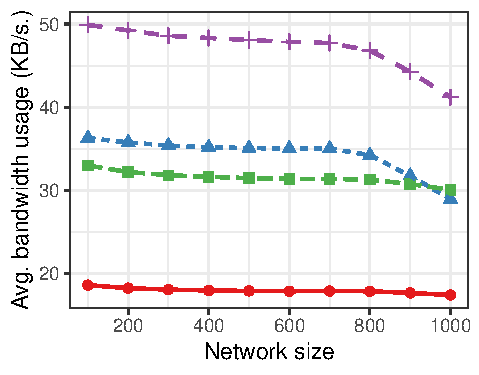
\includegraphics[width=\columnwidth]{trustchain/assets/fraud_experiment_dynamic_tx_bw}
		\caption{Bandwidth usage}
		\label{fig:fraud_experiment_dynamic_tx_bw}
	\end{subfigure}%
	\caption{The fraud detection times and bandwidth usage of \ModelName{} while recording scaling the creation of interactions with the network size. $ n $ indicates the network size. We fix the fanout to 10.}
	\label{fig:fraud_experiments_dynamic_tx}
\end{figure*}

\section{Implementation and Evaluation}
\label{sec:implementation_evaluation}
We implement the \ModelName{} transaction model (section~\ref{sec:micro_accounting}), the micro-record validation logic (Section~\ref{sec:detecting_fraud}) and system architecture (Section~\ref{sec:system_architecture}) in the Python 3 programming language.
We use our existing networking library as communication layer.\footnote{See https://github.com/tribler/py-ipv8}
We adopt an event-driven programming model using the \texttt{asyncio} library.
We use the UDP protocol for data exchange and keep track of outstanding queries using request stores and timeouts.
Our implementation features both an (optimized) in-memory and a \texttt{sqlite} database.
The full implementation of \ModelName{}, including unit tests and documentation, is published on GitHub.\footnote{See https://github.com/tribler/py-ipv8/tree/master/ipv8/attestation/trustchain}

We evaluate \ModelName{} on our nation-wide university cluster which hardware specifications can be found online.\footnote{https://www.cs.vu.nl/das5/clusters.shtml}
Our experiments answer the following questions: (1) how fast can forking be detected with varying network sizes and differing strategies to exchange micro-records? (2) What is the bandwidth usage of \ModelName{} under different exchange strategies? And (3) how does the throughput of \ModelName{} behave under different network sizes and fanout rates?

\subsection{Fraud Detection}
\label{sec:fraud_detection_experiment}
We evaluate the efficiency of detecting forks in \ModelName{} by measuring the time between committing the fraud and its initial detection.
During our experiments, users record fake interactions with random users.
For network sizes from 100 to 1'000 users, we fix our experiment such that each user with a probability of 10\% forks its personal ledger by removing the last micro-record in its micro-record and re-using the sequence number to record a new interaction.
Each user forks its personal ledger once during the experiment.
Each run has a duration of five minutes where all users start with an empty personal ledger, and proposals are always confirmed by the interaction partner.
We run each experiment at least ten times, and average all results.

%The global rate at which transactions are made is fixed to 100 transactions per second.

To analyse the impact of different micro-record exchange strategies on fraud detection time and bandwidth usage, we consider the following four strategies.
With the \texttt{PULL} strategy, each user requests five contiguous micro-records at a random height in the personal ledger of another random user every half a second.
Under the \texttt{PULL+RAND}, user also returns five random micro-records in their database upon a query.
The \texttt{PULL+PUSH} strategy pushes new micro-records to $ f $ random users upon creation.
We fix $ f $ to 10 for all experiments.
Finally, we consider the \texttt{PULL+RAND+PUSH} strategy, which is a combination of the above strategies.
To model adversarial behaviour, users forking their personal ledger refrain from pushing the newly created micro-record to others.
Note that the \texttt{PULL} and \texttt{PULL+RAND} strategies resemble the situation where two interaction partners collaborate to hide the conflicting micro-record since there is no dissemination of these micro-records.

%During the experiment, each peer explores others' personal ledgers by continuously querying their latest micro-record, and attempts to detect fraud.
%At the start of each experiment, we selected one peer to perform exactly one double spend attack.
%This peer re-uses the sequence number of the latest micro-record (forking) with 20\% probability.
%We measure the interval between initiation of the fraud and its first detection (upon which the proof can be spread in the network).
%We vary the rate at which users request micro-records from each other.
%We consider request frequencies of 5, 10 and 25 (where 5 means that each user will request a micro-record from five other users every second).
%For each combination of network size and ledger exploration rate, we run the experiment 20 times.

Figure~\ref{fig:fraud_experiments_fixed_tx} shows the fraud detection times and bandwidth usage while recording 100 interactions per second, for different exchange strategies and network sizes ($ n $).
Figure~\ref{fig:fraud_experiment_fixed_tx_time} reveals that fraud can be detected within ten seconds under all strategies, even when $ n = 1'000 $.
The detection times decrease when enabling a push-based exchange strategy (\texttt{PULL+PUSH}), and when sharing random micro-records during a crawl (\texttt{PULL+RAND}).
Furthermore, the detection times increase roughly linearly when increasing the network size for the \texttt{PULL+PUSH} and \texttt{PULL+RAND+PUSH} strategies.
In Figure~\ref{fig:fraud_experiment_detect_times_fixed_1000}, we show an ECDF of the detection times for different strategy and with $ n = 1'000 $.
Note how 50\% of all fraud attempts is detected within ten seconds.
We notice a significant effect of the push-based exchange strategy on the detection times.
We explain this effect as follows: pushing created micro-records to random users lead to near-immediate detection of fraud when a user receives two conflicting micro-records.
Figure~\ref{fig:fraud_experiment_fixed_tx_bw} shows the average bandwidth consumption of each user during our five-minute runs.
The average bandwidth usage decreases when the network grows which is likely the result of fixing the rate at which new micro-records are created.
With $ n = 1'000 $, the \texttt{PULL+RAND+PUSH} strategy requires 25KB/s. on average and the \texttt{PULL} strategy only requires 14.5 KB/s.

Figure~\ref{fig:fraud_experiments_dynamic_tx} shows the detection times and bandwidth usage while scaling the number of recorded interactions with the network size.
This results in a higher fraud detection times, as hinted by Figure~\ref{fig:fraud_experiment_dynamic_tx_time}.
Still, fraud attempts are detected within reasonable time: even the \texttt{[PULL} strategy enables fraud detection within 22 seconds on average.
Figure~\ref{fig:fraud_experiment_detect_times_dynamic_1000} shows that the effect of individual strategies on fraud detection times is more pronounced under a dynamic micro-record creation rate.
Additionally, Figure~\ref{fig:fraud_experiment_dynamic_tx_bw} shows that the average bandwidth usage remains roughly constant when increasing the network size, but slightly drops for $ n > 800 $.
These experiments show that fraud can be detected efficiently with reasonable bandwidth usage.

%The results are given in Figure \ref{fig:fraud_experiment}.
%The horizontal axis denotes the network size and the vertical axis shows the time interval between performing the forking and its detection.
%The errors bars show one standard deviation of uncertainty.
%Figure \ref{fig:fraud_experiment} shows that faster querying of micro-records increases the speed of fraud detection, at the expense of increased resources usage (bandwidth and CPU utilization).
%We observe that the variation of fraud detection speed is higher when exploring personal ledgers at a lower rate.
%Interesting is that effectiveness of fraud detection shows comparable results when the network size increases.
%Our reasoning for this is as follows: although the specific double spend is more "hidden" in the network, there is also more ongoing effort to detect it.
%This experiment shows that forking of a personal ledger can be detected within mere seconds and 1'000 active peers.

\begin{figure}[b]
	\centering
	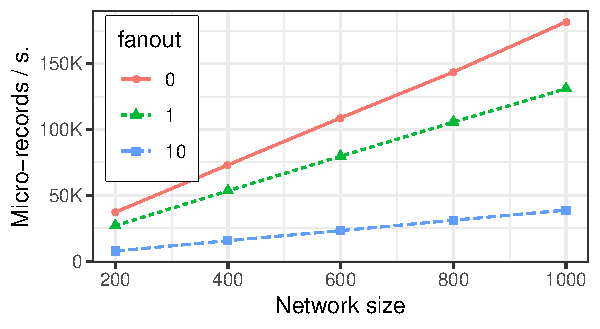
\includegraphics[width=\linewidth]{trustchain/assets/scalability}
	\caption{The rate at which we can create new micro-records in \ModelName{} when increasing the network size.}
	\label{fig:scalability}
\end{figure}

\subsection{Scalability}
We explore the scalability of \ModelName{} by having each user recording an interaction with another random user at a fixed interval.
After creating a micro-record, it is disseminated to $ f $ random users, where $ f $ is the fanout.
We systematically explore the maximum creation rate of micro-records for different network sizes and fanout rates during 30-seconds experiment runs.
For each value of $ n $ and $ f $, we report the highest throughput achieved.
We use the in-memory database during this experiment.

The results of our scalability experiment are presented in Figure~\ref{fig:scalability}, with the network size on the horizontal axis and the maximum micro-record creation rate on the vertical axis.
\ModelName{} is able to create 181'729 confirmed micro-records per second with 1'000 peers and $ f = 0 $.
During this run, the average bandwidth usage per peer is 121 KB/s.
A higher fanout negatively affects the throughput: with $ f = 10 $ and $ n = 1'000 $, \ModelName{} outputs 38'810 confirmed micro-records per second.
Figure~\ref{fig:scalability} hints at linear scalability when the network size grows and $ f $ remains fixed.
We remark that our current implementation is single-threaded and the achievable throughput can still be improved by leveraging parallelism.
The current throughput of \ModelName{}, however, should be sufficient for many deployed shared-resource systems.

\section{Addressing Free-riding at Scale}
\label{sec:deployment}
To show the practicality and matureness of \ModelName{}, we conduct a large-scale deployment trial with to address free-riding behaviour in our academic file-sharing software named \Tribler{}.
\Tribler{} is downloaded by over 1.5 million users and features an onion-routing overlay that tunnels BitTorrent traffic through relay and exit nodes to provide anonymity.
This overlay suffers from an undersupply of exit nodes, leading to frequent network congestions and an overall degradation of download speeds for all users.
We leverage \ModelName{} to account bandwidth contributions as relay or exit node, and consumptions as downloader.
We demotivate free-riding behaviour by offering users with higher net contributions preferential treatment during periods of congestion.

\begin{figure}[t]
	\centering
	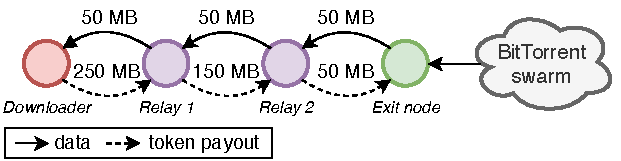
\includegraphics[width=\linewidth]{trustchain/assets/payouts}
	\caption{Accounting an anonymous 50MB BitTorrent download using \ModelName{} and a two-hop onion-routing circuit.}
	\label{fig:payouts}
\end{figure}

\subsection{Accounting Bandwidth Transfers}
With \ModelName{}, each user earns \emph{bandwidth tokens} by forwarding traffic as a relay or exit node.
When downloading content, the user compensates the used relay and exit nodes.
Figure~\ref{fig:payouts} show how a downloader pays tokens to others nodes after downloading a 50 Megabyte file over a two-hop circuit.
When the circuit is destroyed, the downloader accounts a transfer of 250MB to the first relay node using \ModelName{} (MB is the unit of this bandwidth token).
The first relay node then transfers 150MB to the next relay node, earning 100MB.
The rationale behind our payout scheme is that we reward relay and exit nodes for performing the cryptographic operations on the forwarded data.
Relays that do not forward the payout to the next hop will be blacklisted by the previous hop, lowering their opportunity to earn bandwidth tokens.
Each micro-record in a personal ledger contains the token amount transferred in that interaction, and the current token balance of the user.
%We payout anonymous transfers of at least 1MB.

We remark that there is a trade-off between accountability and anonymity.
We plan on addressing privacy concerns by having each node aggregate and delay payouts, a privacy-enhancing technique introduced in the work of Palmieri et al. ~\cite{palmieri2015paying}.
Still, bandwidth accounting with \ModelName{} currently does not leak the identity of a downloader to others, nor reveals the data being exchanged.
To address the uncontrolled minting of bandwidth tokens by recording fake interactions, we are currently designing and implementing a Sybil-resistant reputation mechanism~\cite{otte2017trustchain}.

\begin{algorithm}[t]
	\label{alg:slot_logic}
	\caption{The assignment logic of slots to circuits. $ r $ and $ c $ represent the number of random and competitive slots, respectively.}
	\begin{algorithmic}[1]
		\State randomSlots $ \leftarrow [0] * r $ \Comment{array with circuit IDs}
		\State competitiveSlots $ \leftarrow [(-1, 0)] * c $ \Comment{array with balances and circuit IDs}
		\State
		
		\Function{onCircuitRequest}{circuit}
		\For{index, circuitId \textbf{in} enumerate(randomSlots) }
		\If{circuitId $ = $ 0}
		\Comment{Random slot is available}
		\State randomSlots[index] = circuit.id
		\State \textsc{notify}(circuit)
		\State \Return
		\EndIf
		\EndFor
		
		\State \textsc{requestCreatorBalance}(circuit)
		
		\EndFunction
		\State
		
		\Function{onBalance}{circuit, creatorBalance}
		\State lowestBalance = $ \infty $
		\State lowestIndex = 0
		\For{index, circuitId, balance \textbf{in} randomSlots }
		
		\If{circuitId $ = $ 0} \Comment{Comp. slot is available}
		\State randomSlots[index] = (circuit.id, creatorBalance)
		\State \textsc{notify}(circuit)
		\State \Return
		\EndIf
		
		\If{balance $ < $ lowestBalance}
		\State lowestBalance $ = $ balance
		\State lowestIndex $ = $ index
		\EndIf
		\EndFor
		
		\If{creatorBalance $ > $ lowestBalance}
		\State \textsc{kick}(lowestIndex)
		\State randomSlots[index] = (circuit.id, creatorBalance)
		\State \textsc{notify}(circuit)
		\State \Return
		\EndIf
		
		\EndFunction
		
	\end{algorithmic}
\end{algorithm}

\begin{figure*}[t]
	\centering
	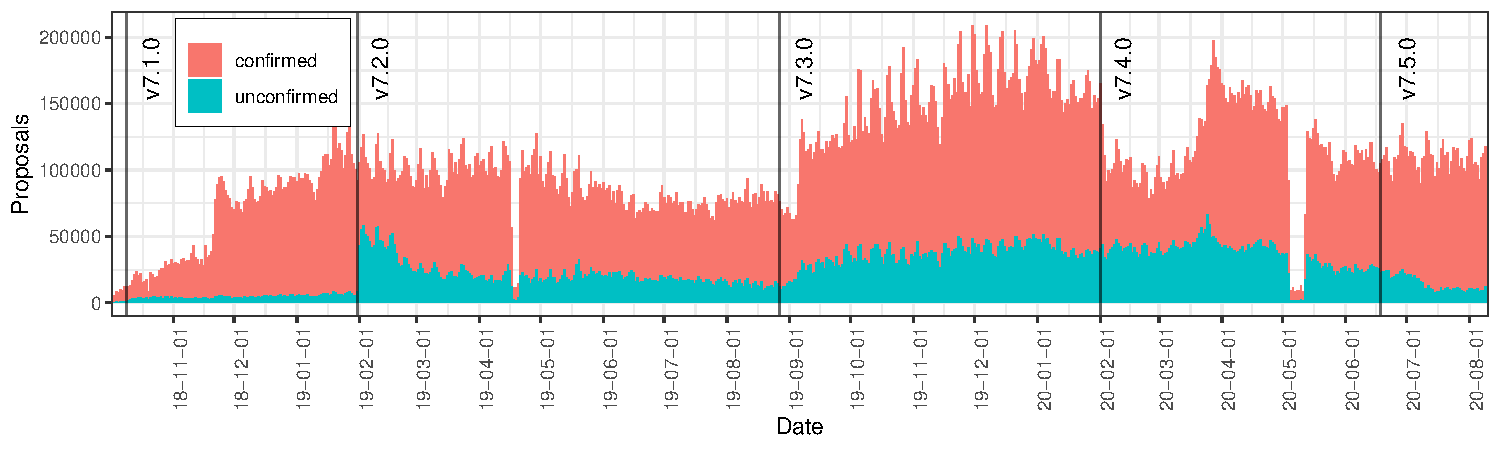
\includegraphics[width=\linewidth]{trustchain/assets/record_creation}
	\caption{Daily creation statistics of micro-records, since we deployed our \ModelName{} crawler. We annotate the major releases of \Tribler{}.}
	\label{fig:record_creation}
\end{figure*}

We grant preferential treatment to users with higher token balances during congestion.
To do so, we modify relay and exit nodes such that each circuit consumes an available slot at their side.
The slot assignment process is listed in Listing~\ref{alg:slot_logic}.
We distinguish between \emph{random} and \emph{competitive} slots.
When a circuit initiation request arrives, the \texttt{onCircuitRequest} method is invoked and \Tribler{} first determines if there is a random slot available.
If so, we assign the new circuit to the random slot.
If no random slot is available, \Tribler{} queries the bandwidth token balance of the circuit initiator $ i $ by invoking the \texttt{requestCreatorBalance} which requests the micro-records in the personal ledger of $ i $.
When receiving these micro-records, the balance is determined and \Tribler{} now checks eligibility for a competitive slot.
If there is an unoccupied competitive slot, \Tribler{} assigns the new circuit to it.
If all competitive slots are filled, the circuit of the initiator with the lowest amount of bandwidth tokens, say $ p $, is destroyed if the token balance of $ i $ is higher than the token balance of $ p $.
This pre-emptive approach frees up the competitive slot for the circuit of $ i $.
As a result, users with a higher token balance have more chance to claim a competitive slot in periods of congestion, compared to free-riders, and thus they experience higher and more stable download speeds.

\begin{figure}[b]
	\centering
	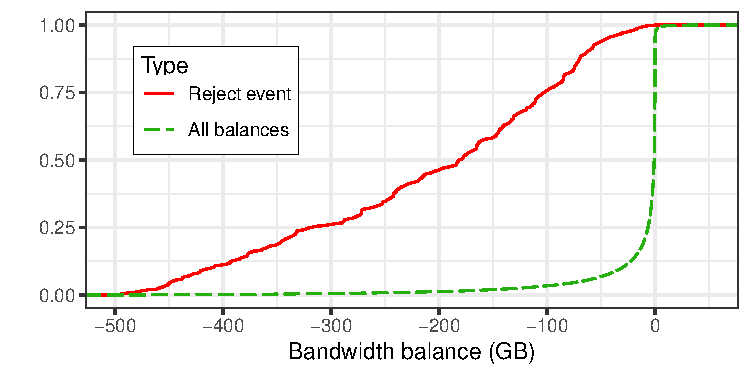
\includegraphics[width=\linewidth]{trustchain/assets/exit_node_rejects}
	\caption{ECDF showing the distribution of bandwidth token balances users and individual rejects events at exit nodes.}
	\label{fig:exit_node_rejects}
\end{figure}

%\begin{figure}[t]
%	\centering
%	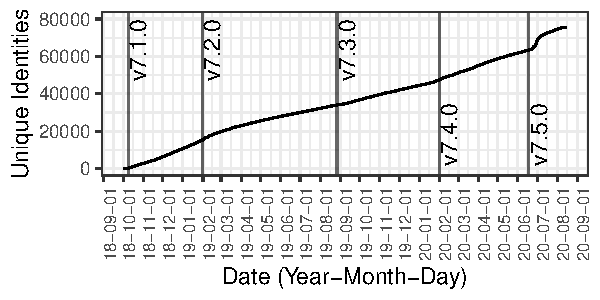
\includegraphics[width=\linewidth]{assets/identities_per_day}
%	\caption{ECDF showing the distribution of bandwidth token balances users and individual rejects events at exit nodes.}
%	\label{fig:identities_per_day}
%\end{figure}

\subsection{Data Collection}
We implement the accounting and slot mechanism in \Tribler{} and release a new version of our software.
We also deploy a crawler that fetches \ModelName{} micro-records from random users in the \Tribler{} network.
Every two seconds, this crawler selects a random user in the network and requests missing micro-records in their personal ledger.
This has resulted in more than \TrialRecords{} micro-records, created by over \TrialUsers{} individuals during our deployment period (36 months).
These micro-records are stored in a sqlite database that is enhanced with additional indices to speed up analysis queries.
The filesize of the database with all micro-records is around 100GB.
In addition, our crawler discovered 127'135 instances where a personal ledger was forked.

Monitoring the micro-records created by \ModelName{} not only allows us to detect free-riders but it also allows us to detect network anomalies caused by software bugs or network outages.
Furthermore, it enables us to make estimations on the user growth of our network.
To this end, we include a timestamp in the payload of each micro-record, which is the clock time of the user.
We acknowledge that this timestamp might be inaccurate, however, it yields a rough overview of the network dynamics over time.

Figure~\ref{fig:record_creation}, shows the daily number of created proposals and confirmations.
We also annotate the dates on which we released a major version of \Tribler{}.
Note that it could be that an unconfirmed micro-record as reported by the crawl might have been confirmed, but the crawler may not have picked it up from the network, e.g., because the interaction partners went offline.
Figure~\ref{fig:record_creation} shows how the rate at which micro-records are created varies within a week period.
In particular, we find that more users run \Tribler{} during the weekend and therefore create more proposals.
We also observed two large-scale outage of exit nodes, in April 2019 and May 2020.
Despite this outage, users would still perform payouts when downloading directly from other \Tribler{} users, showing the robustness of \ModelName{}.
%Note how major release of \Tribler{} is not significantly resulting in an increased number of micro-records.

In \Tribler{}, users earn bandwidth tokens by either operating an exit node, or by relaying traffic.
By default, users download with one-hop anonymity, meaning that the circuit is directly connected to an available exit node.
We noticed that only few users increase this setting since adding additional hops to a circuit negatively impacts the achievable download speed.
%There is a delicate trade-off between anonymity and download speed. 
Therefore, there is an oversupply of relay nodes but the majority of users do not require a relay node for their downloads.
Eventually, we aim to adjust the default number of hops for a download to two, increasing the opportunities for relay nodes to earn bandwidth tokens.
%We are currently improving the performance of our anonymous download mechanism.

\subsection{Free-rider Identification and Service Refusal}
To evaluate whether free-riding behaviour is addressed, we support the \Tribler{} network with 48 additional exit nodes.
Each exit node has a total of 10 random slots and 20 competitive slots, resulting in a total of 1'440 slots.
We log the bandwidth token balance when a circuit initiator is unable to claim a competitive slot at one of our exit nodes.
In total, we logged over 1.2 million reject events during three weeks.

Figure~\ref{fig:exit_node_rejects} shows an ECDF with the bandwidth token balances of all users (dotted green line) and the balances of reject events (solid red line).
We filter out all users and reject events with balances higher than 50GB or lower than -500GB.
The median token balance of all users is -713MB and that of reject events -181.4GB, demonstrating that our mechanism targets users with lower balances.
In other words, long-term free-riders are more likely to be kicked out when the network is congested.
This deployment trial shows that \ModelName{} is effective at detecting and addressing free-riding behaviour in \Tribler{}.
On the long term, the integration of \ModelName{} increases network performance and induces fairness amongst downloading users.

%\begin{figure}[t]
%	\centering
%	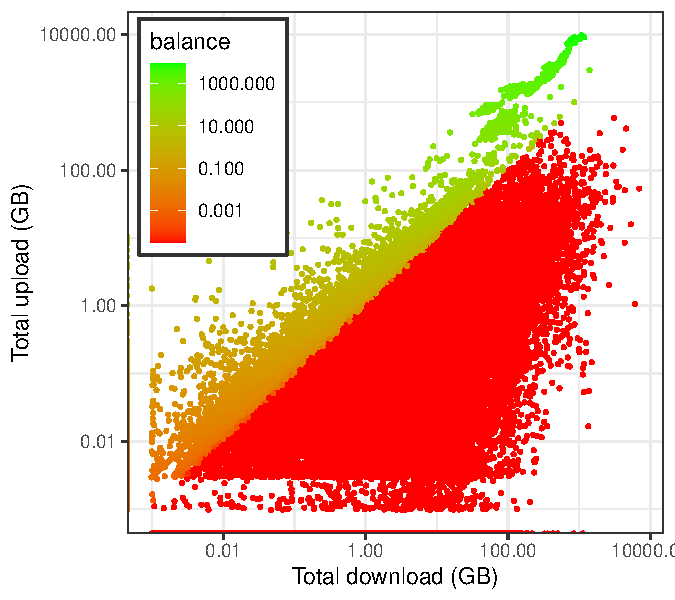
\includegraphics[width=\linewidth]{assets/balances_scatter}
%	\caption{The bandwidth balances of users in Tribler. Users with a balances less than 5GB are marked red.}
%	\label{fig:balances}
%\end{figure}

\section{Related Work}
Wallach et al., present different mechanisms for fair sharing of peer-to-peer resources, however, their work exclusively focusses on storage-based systems~\cite{wallach2003enforcing}.
To the best of our knowledge, their design is not compatible with multiple shared-resource system, limiting the applicability of their work.
Similarly, the work of Osipkov et al., describe an accounting mechanism for peer-to-peer systems~\cite{osipkov2006robust}.

LiFTinG and AcTinG are protocols for tracking free-riding behaviour in gossip-based systems~\cite{guerraoui2010lifting,mokhtar2014acting}.
The Lifting protocol exploits the message dynamics between peers, e.g., that the content received by a peer is further propagated following the protocol, and uses a statistical approach and cross-checking to detect free-riding peers.
The protocol assumes a randomly connected network topology, however, shared-resource systems might not have such message dynamics.
Similar to \ModelName{}, users in AcTinG maintain a secure log with incoming and outgoing messages.

There have been various proposals to leverage distributed ledger technology for logging purposes.
Vegvisir is a partition-tolerant blockchain designed for power-constrained IoT environments~\cite{karlsson2018vegvisir}.
Their design, unlike \ModelName{} targets permissioned networks.
PeerReview is an accountability system to record message exchange between peers, dedicated witnesses to detect whether a peer deviates from the protocol~\cite{haeberlen2007peerreview}.
In PeerReview, each node is associated with a set of other nodes who act as its witness. A witness periodically audits the chain of its associated users.
PeerReview, however, is unsuitable to deploy in open, large-scale and dynamic shared-resource systems like BitTorrent where users frequently join and leave.
The FullReview protocol extends PeerReview, tracks selfish nodes and evaluates its effectiveness in the context of onion routing~\cite{diarra2014fullreview}.
%Their work also describes an experiment that shows how free-riding behaviour in multicast can be detected.

Otte et al., present TrustChain, a Sybil-resistant reputation mechanism that uses a decentralized accounting mechanism~\cite{otte2017trustchain}.
However, liveness in TrustChain is limited.
Specifically, users in TrustChain cannot engage in the recording of multiple interactions simultaneously, limiting achievable throughput and enabling a denial-of-service attack.
Crosby et al., presents a data structure for tamper-evident logging~\cite{crosby2009efficient}.
This structure is primarily focussed on the logging of unilateral events, whereas \ModelName{} is optimized to account peer-to-peer interactions.

% Tor accounting
There has been considerable effort to incentivize relay and exit node operators in the Tor network.
One of the earlier approaches is Gold Star where directory servers keep track of users providing good services to the community~\cite{dingledine2010building}.
Other approaches like BRAIDS and LIRA, reward relay and exit nodes with credits that can be redeemed for prioritized traffic~\cite{jansen2010recruiting,jansen2013lira}.
These solutions assume a centralized bank or a group of semi-trusted nodes for credit management.
TorCoin proposes a mechanism where relay and exit nodes \enquote{mine} a Bitcoin-derived cryptocurrency but relies on a centralized server for circuit management.~\cite{ghosh2014torpath}.
Several shared-resource systems build on blockchain technology and use monetary incentives to provide communal services, e.g., storage (Filecoin~\cite{benet2018filecoin}) and BitTorrent bandwidth (BitTorrent token~\cite{bittorrenttoken}).

%\begin{figure}[t]
%	\centering
%	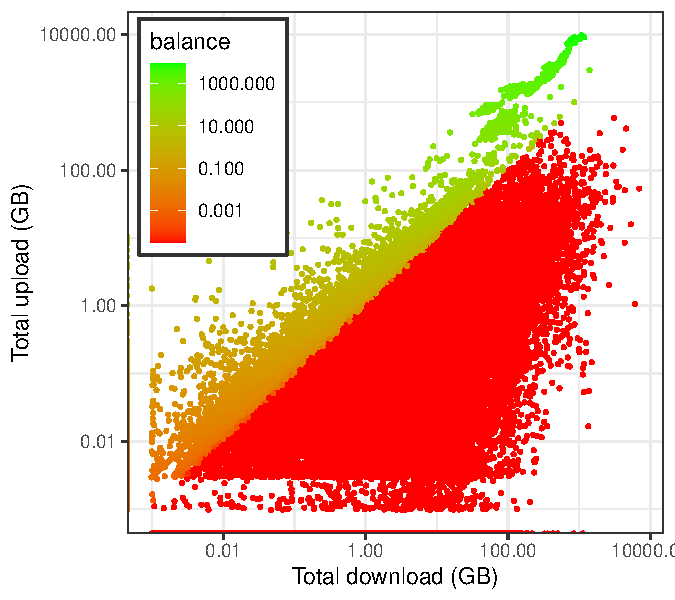
\includegraphics[width=\linewidth]{assets/balances_scatter}
%	\caption{Scatterplot of user balances where each point represents a user in \Tribler{}.}
%	\label{fig:balances_scatter}
%\end{figure}

\section{Conclusion}
We have presented \ModelName{}, a universal accounting mechanism to prevent free-riding in shared-resource systems.
The \ModelName{} data structure uses micro-records and hash pointers to capture bilateral interactions.
Each user maintains a tamper-evident personal ledger.
Forking of a personal ledger is detected by the exchange and validation of micro-records.
We have implemented \ModelName{} and have demonstrated with experiments that our mechanism detects forking within seconds and is highly scalable.
A large-scale deployment trial, involving over \TrialUsers{} users, demonstrated how \ModelName{} addresses free-riding in our peer-to-peer software.

We envision and encourage the usage of \ModelName{} beyond accounting in shared-resource systems.
Currently, \ModelName{} is being tested in different scenarios that require accountability, including decentralized trading and self-sovereign identity~\cite{de2020xchange,stokkink2018deployment}.
These applications have different security requirements compared to shared-resource systems which affects the parameters of \ModelName{} when deployed in these environments, e.g., the rate at which micro-records are exchanged.

%\bibliographystyle{plain}
%\bibliography{references}

\newpage

\appendix

\section{The validation of micro-record data}
\label{sec:validation_record_data}

\begin{algorithm}[h]
	\label{alg:record_data_validation}
	\caption{The validation of the fields in a micro-record.}
	\begin{algorithmic}[1]
		
		\State GenesisSeq $ \leftarrow $ 1
		\State PrevGenesisHash $ \leftarrow $ null
		\State
		
		\Procedure{validateRecordFields}{r}  \Comment{Step 1}
		\If{r.seqNum $ < $ GenesisSeq}
		\State \Return False
		\EndIf
		\If{r.isConfirmation \textbf{and} r.linkSeqNum $ < $ GenesisSeq}
		\State \Return False
		\EndIf
		\If{!\textsc{isValidPublicKey}(r.publicKey)}
		\State \Return False
		\Else
		\If{!\textsc{hasValidSignature}(r)}
		\State \Return False
		\EndIf
		\EndIf
		\If{!\textsc{isValidPublicKey}(r.linkPublicKey)}
		\State \Return False
		\EndIf
		\If{r.seqNum $ = $ GenesisSeq \textbf{and} r.prevHash $ \not= $ PrevGenesisHash}
		\State \Return False
		\EndIf
		\EndProcedure
		
	\end{algorithmic}
\end{algorithm}